\newpage
\section{Appendix}
\label{sec:appendix}

\begin{figure}[h]
    \centering
    \frame{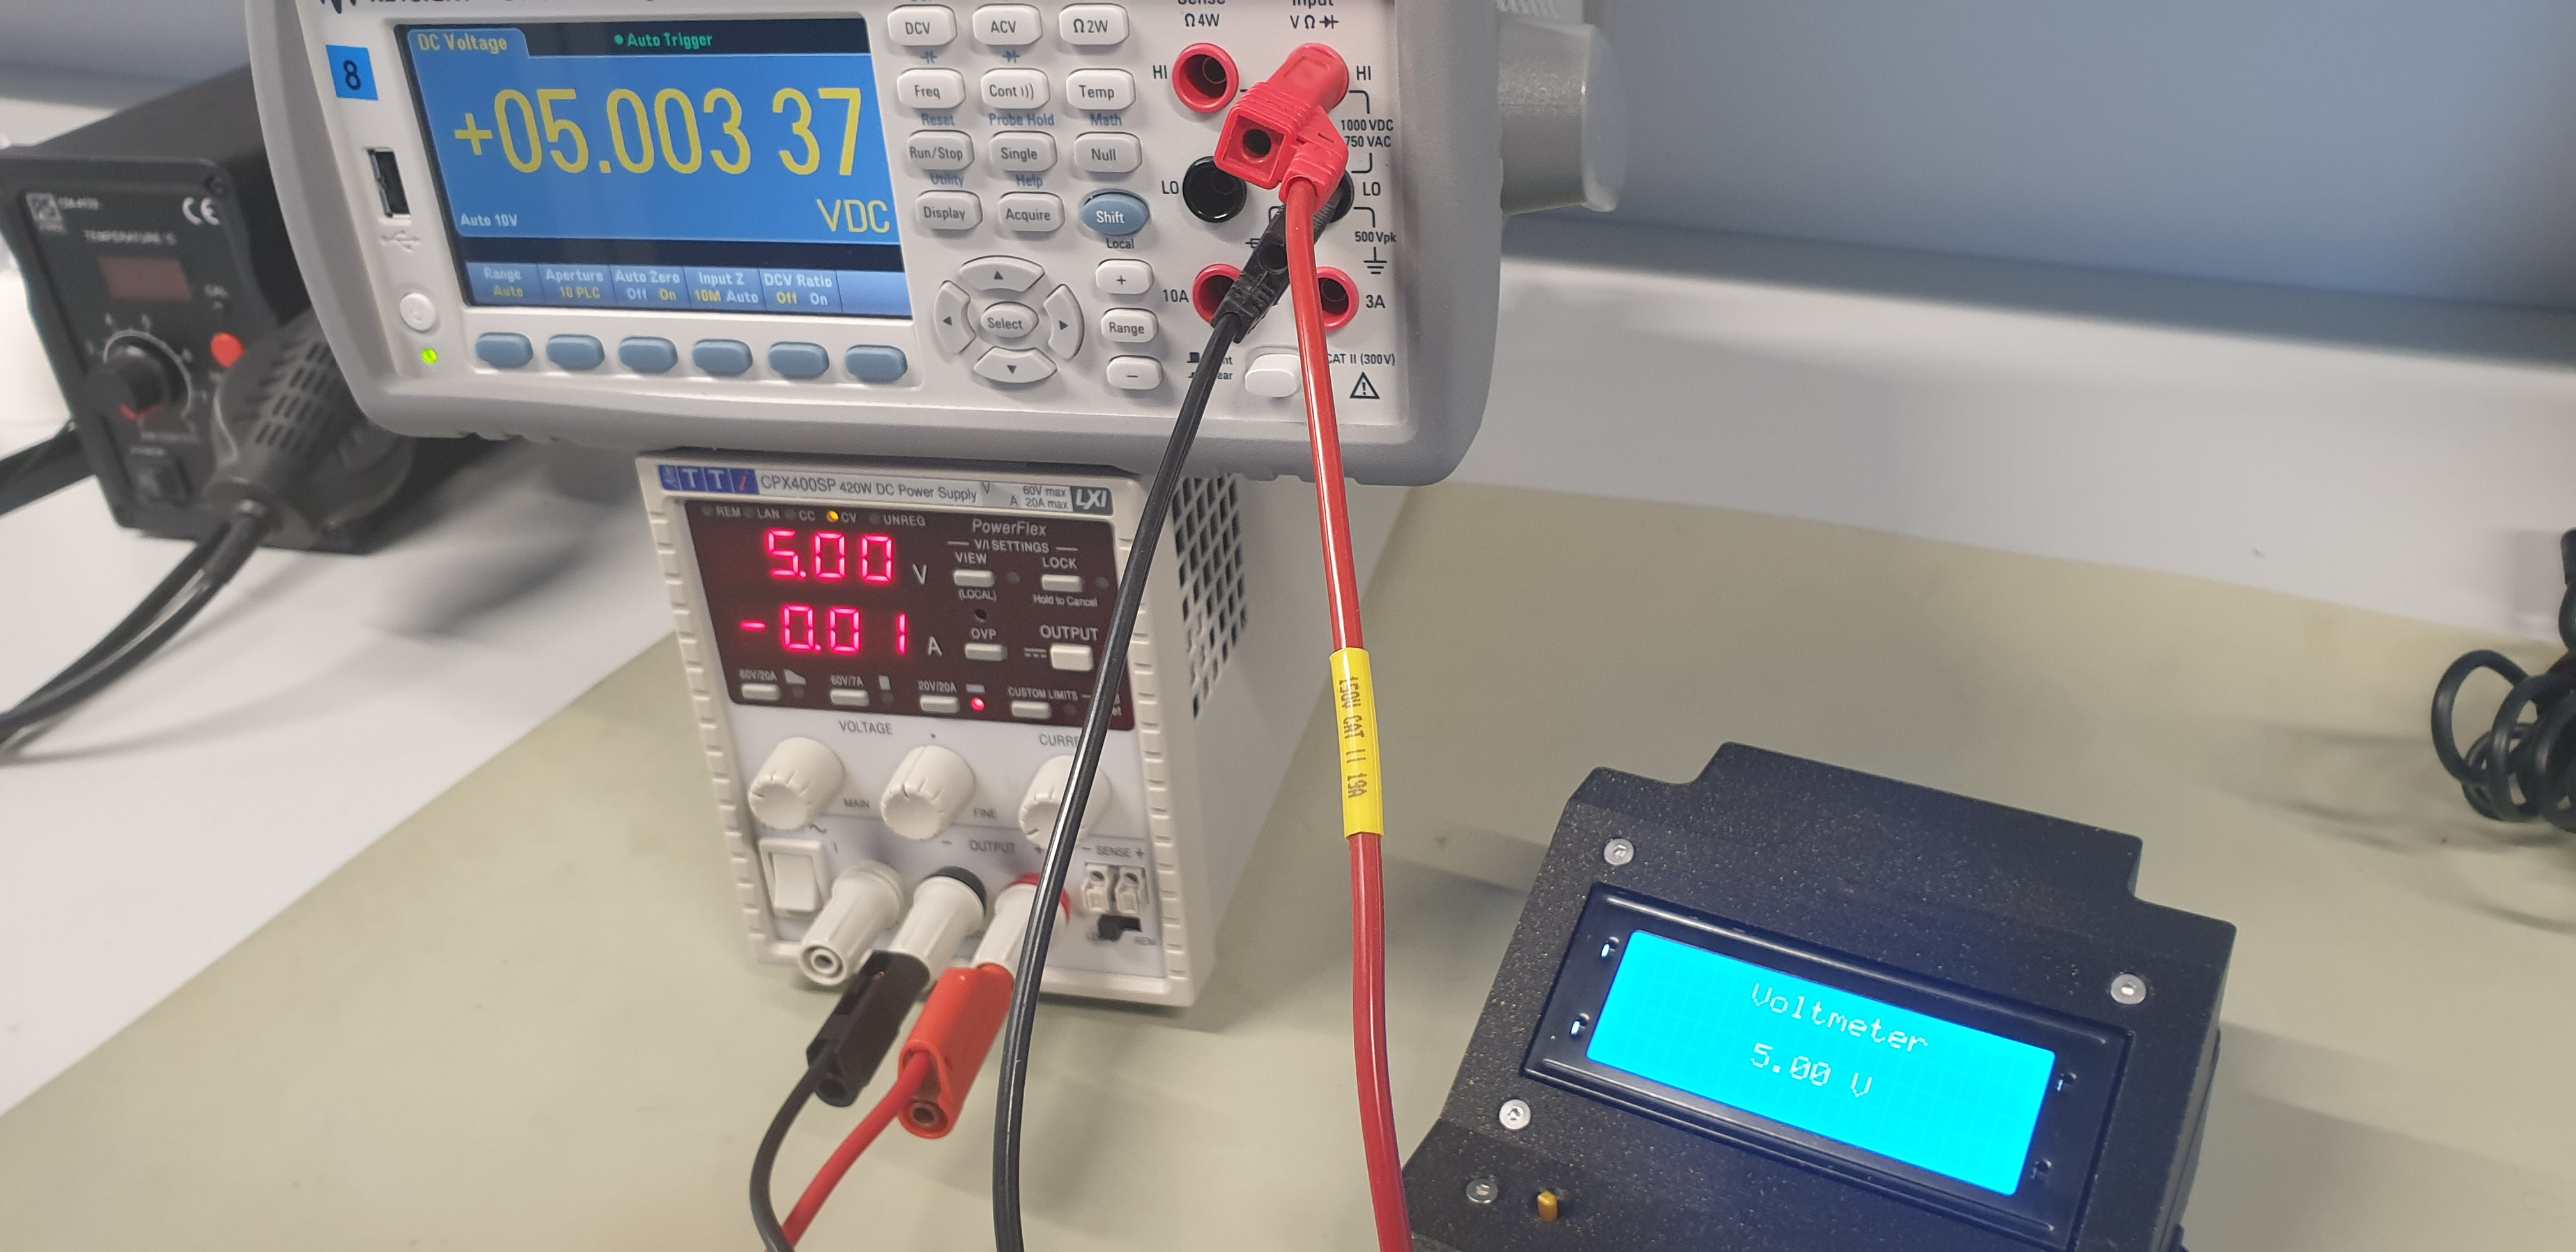
\includegraphics[height=5cm]{images/Measure/VTset.jpg}}
    \caption{Voltage test setup, showing 5V}
    \label{fig:VM1}
\end{figure}

\begin{figure}[h]
    \centering
    \frame{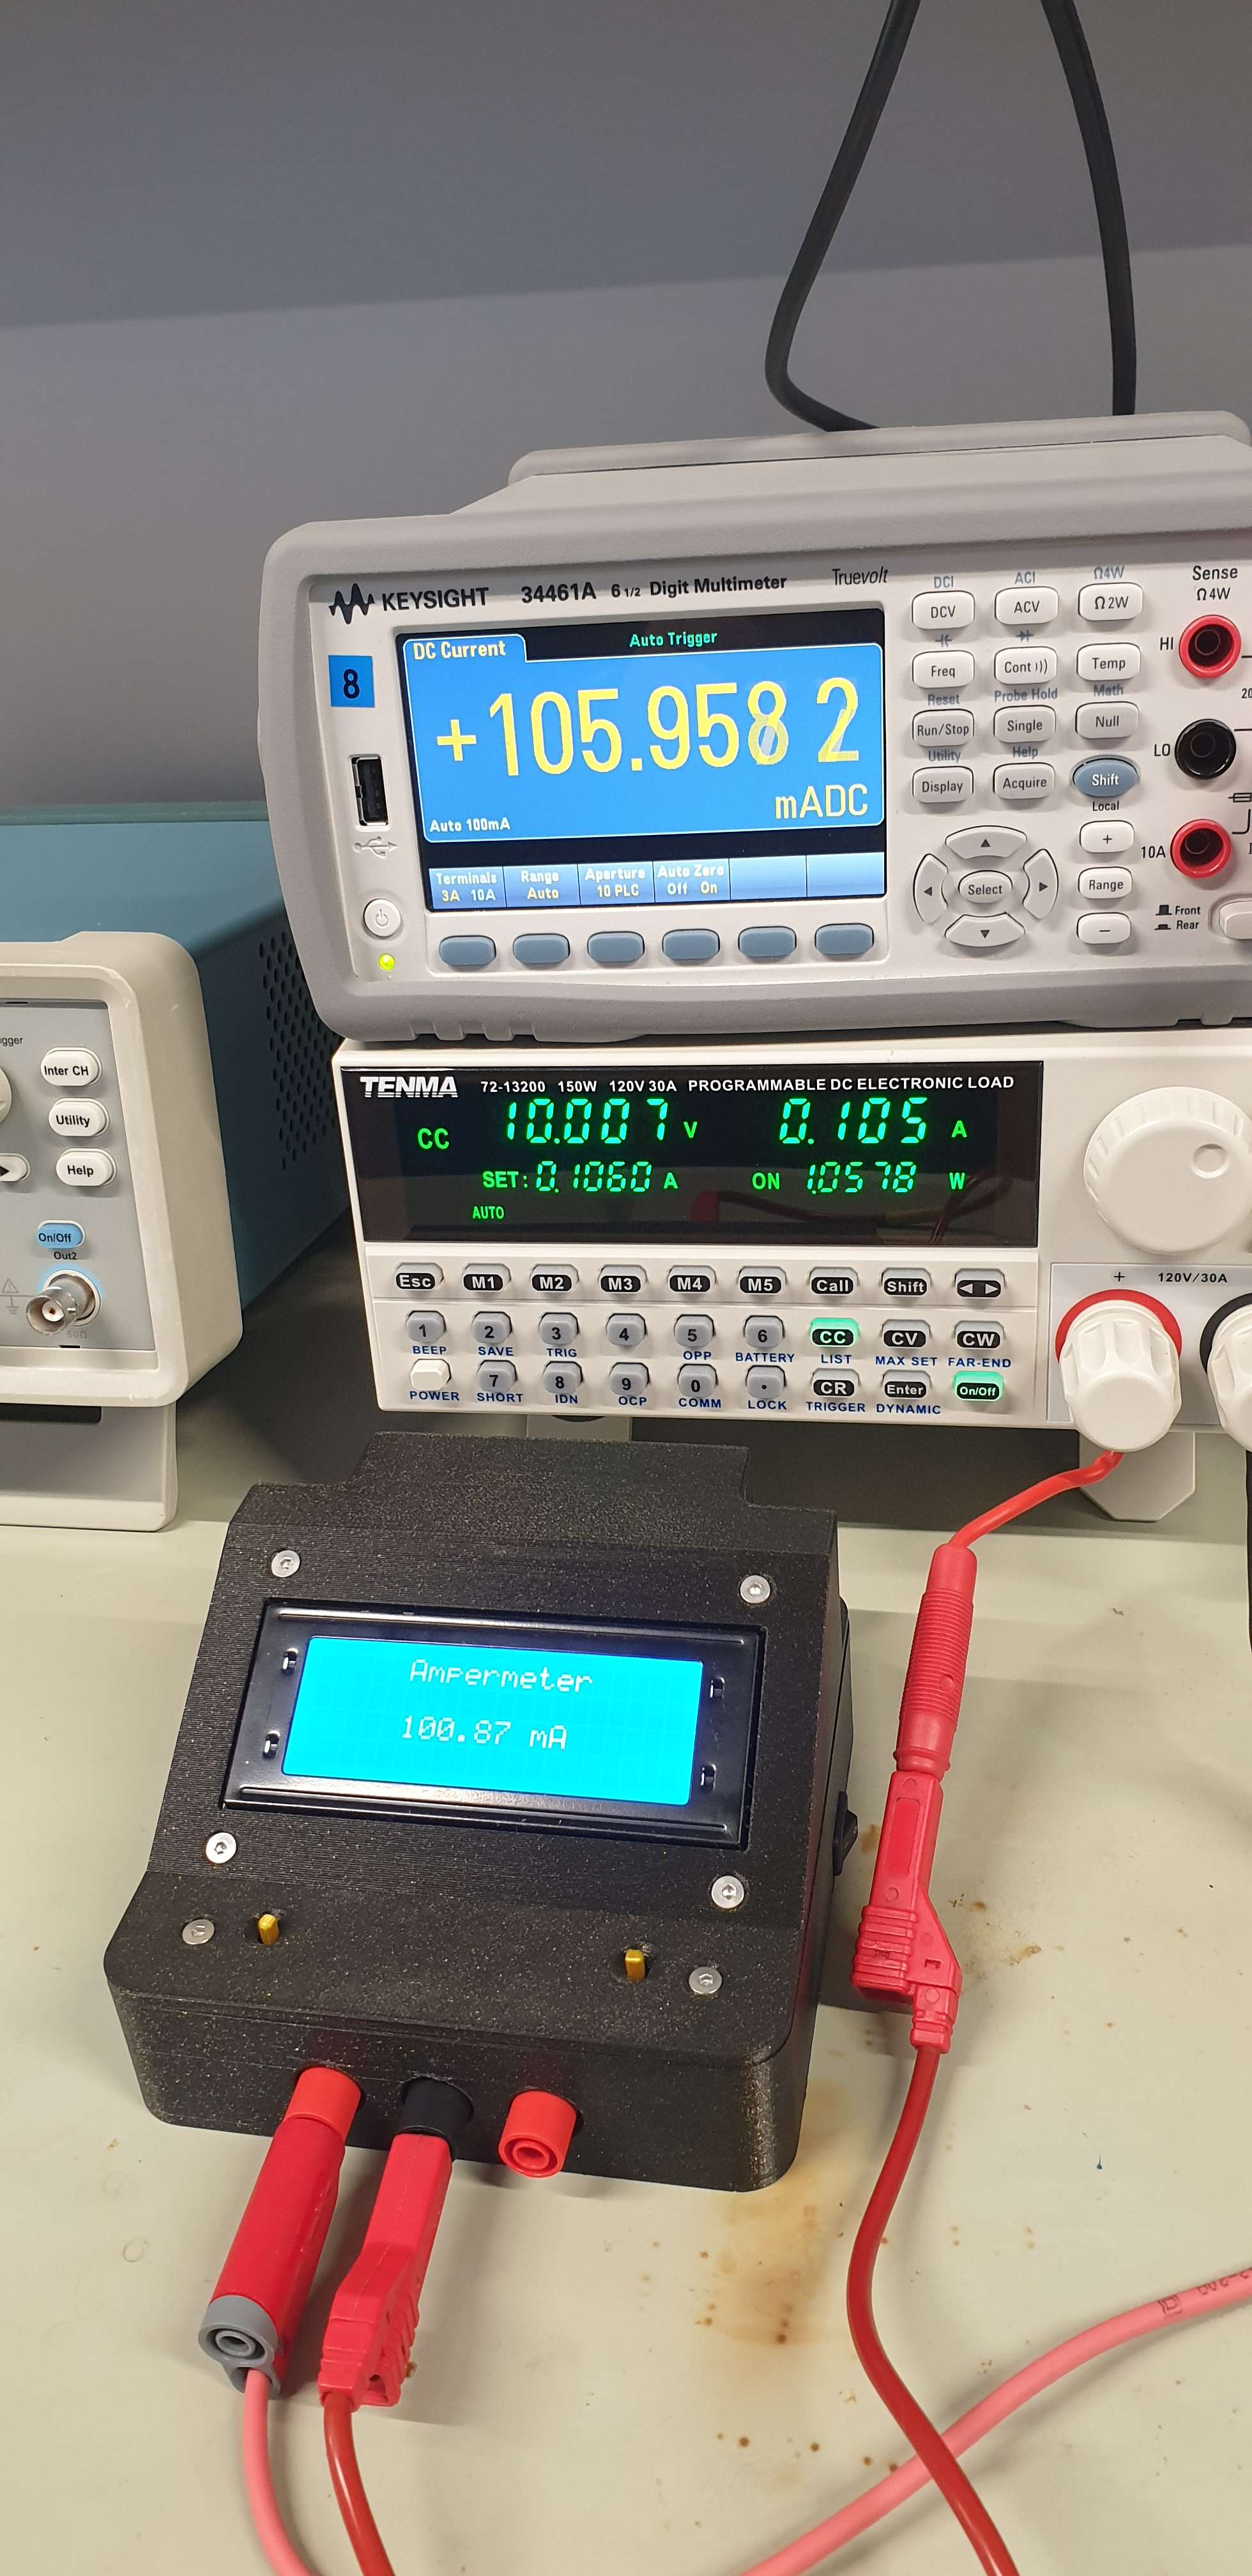
\includegraphics[height=7cm]{images//Measure/currMeas1.jpg}}
    \caption{Current test setup, min value}
    \label{fig:CM1}
\end{figure}

\begin{figure}[h]
    \centering
    \frame{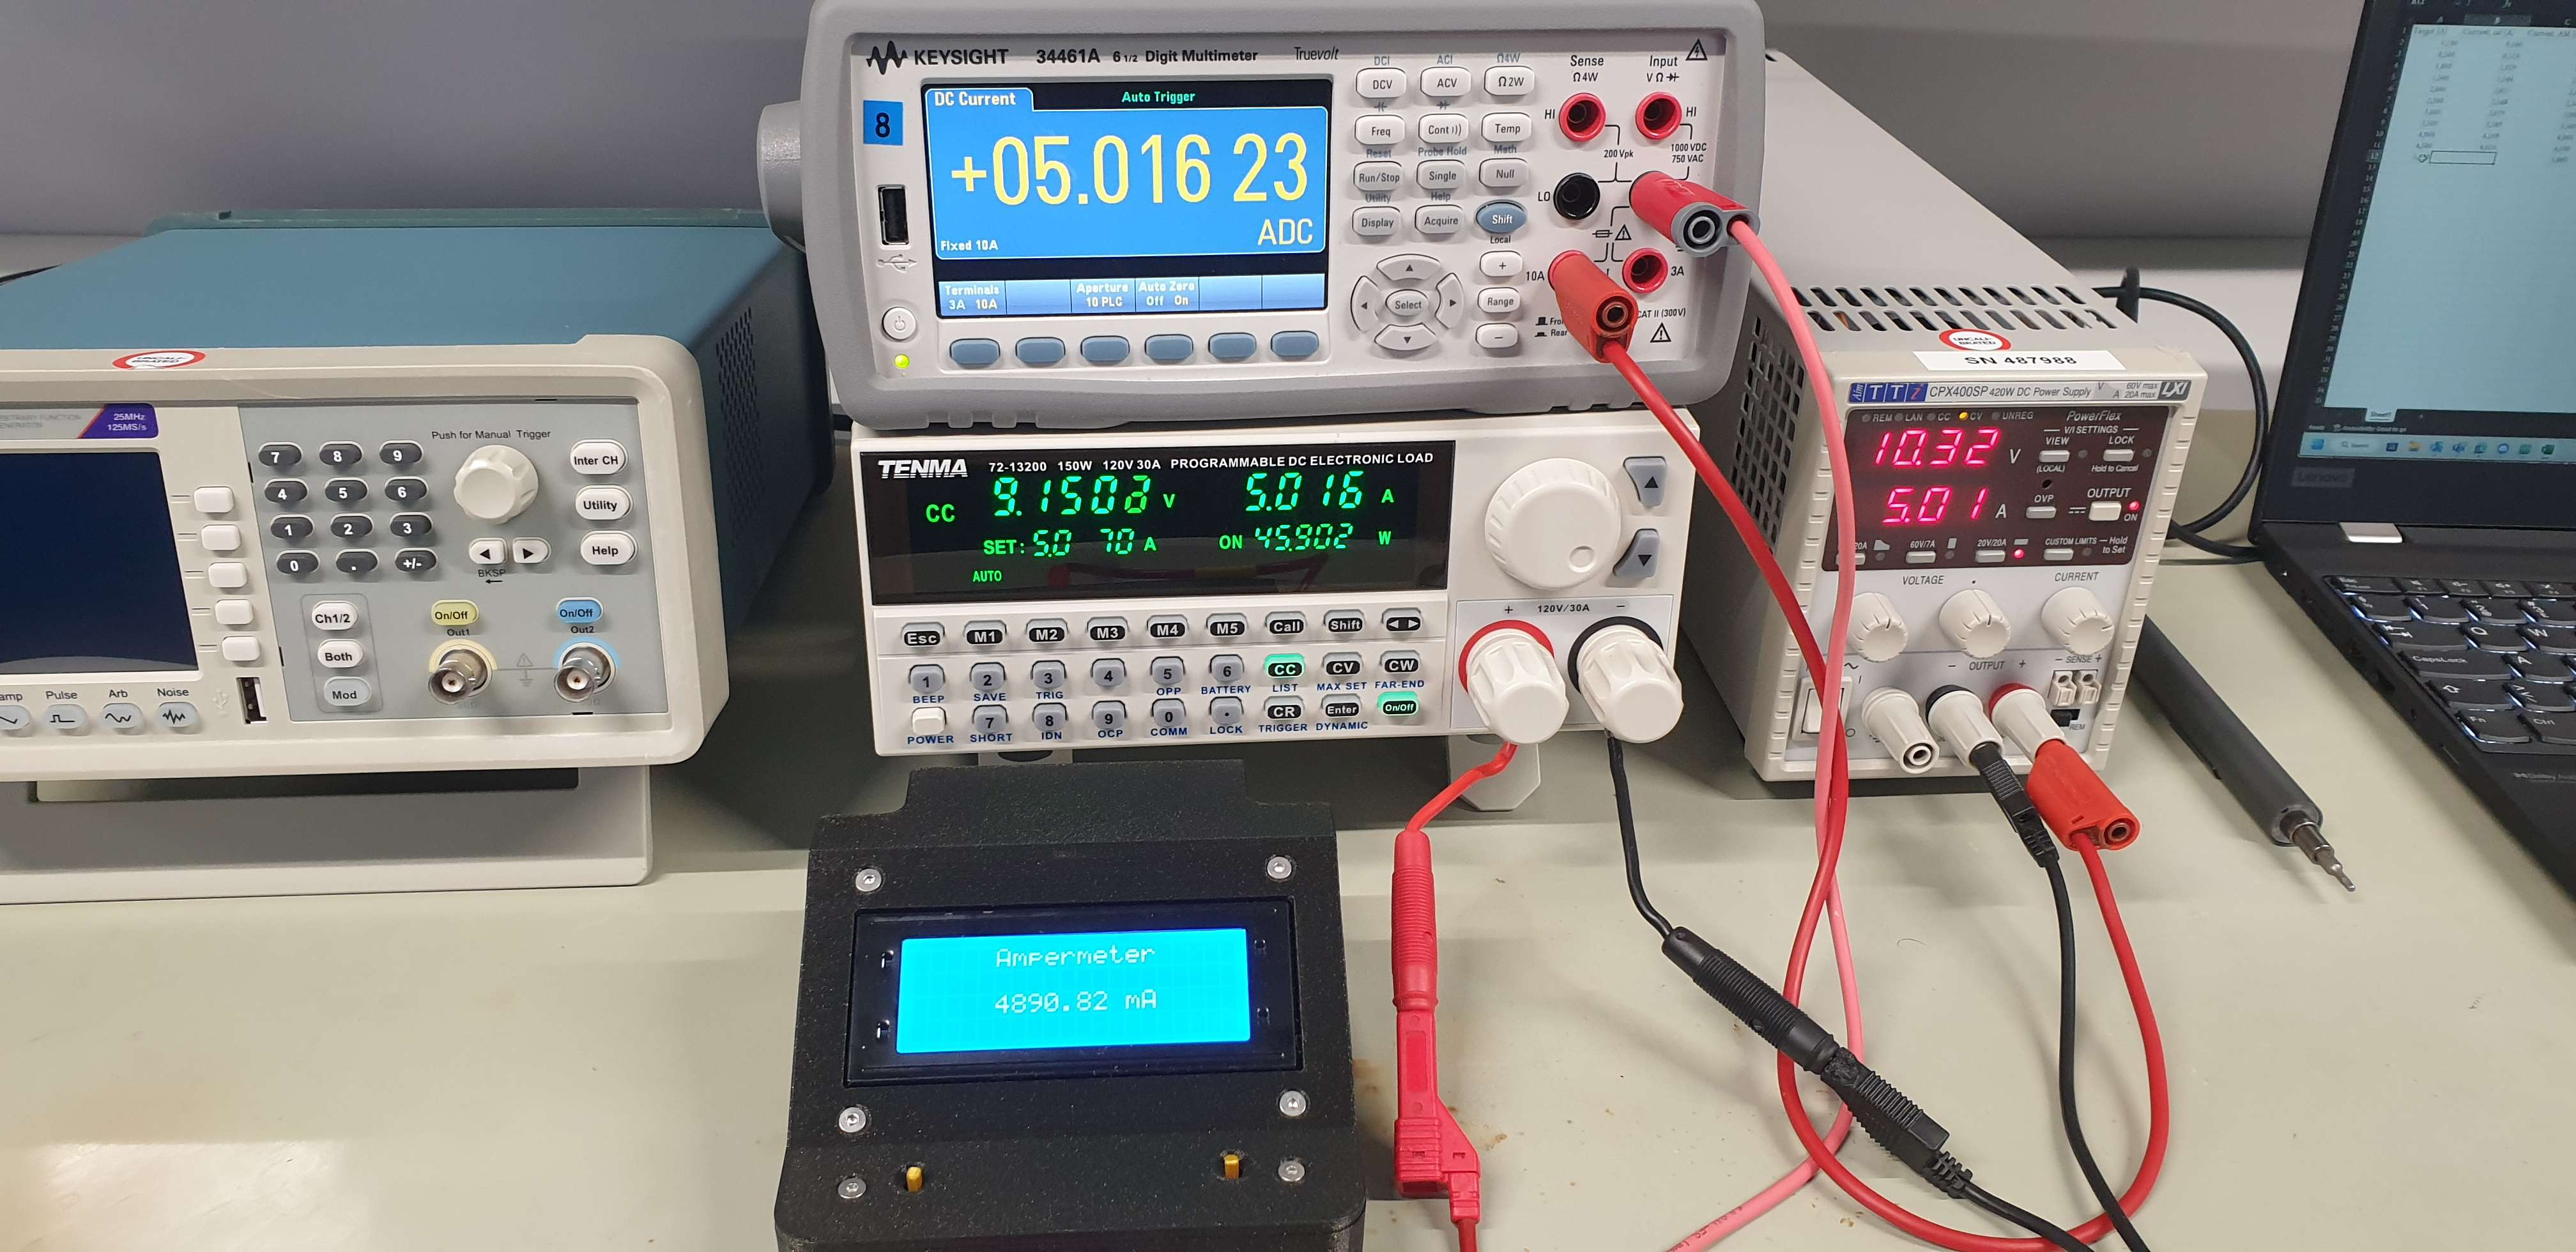
\includegraphics[height=5cm]{images//Measure/currMeas2.jpg}}
    \caption{Current test setup, max value}
    \label{fig:CM2}
\end{figure}

\begin{figure}[h]
    \centering
    \frame{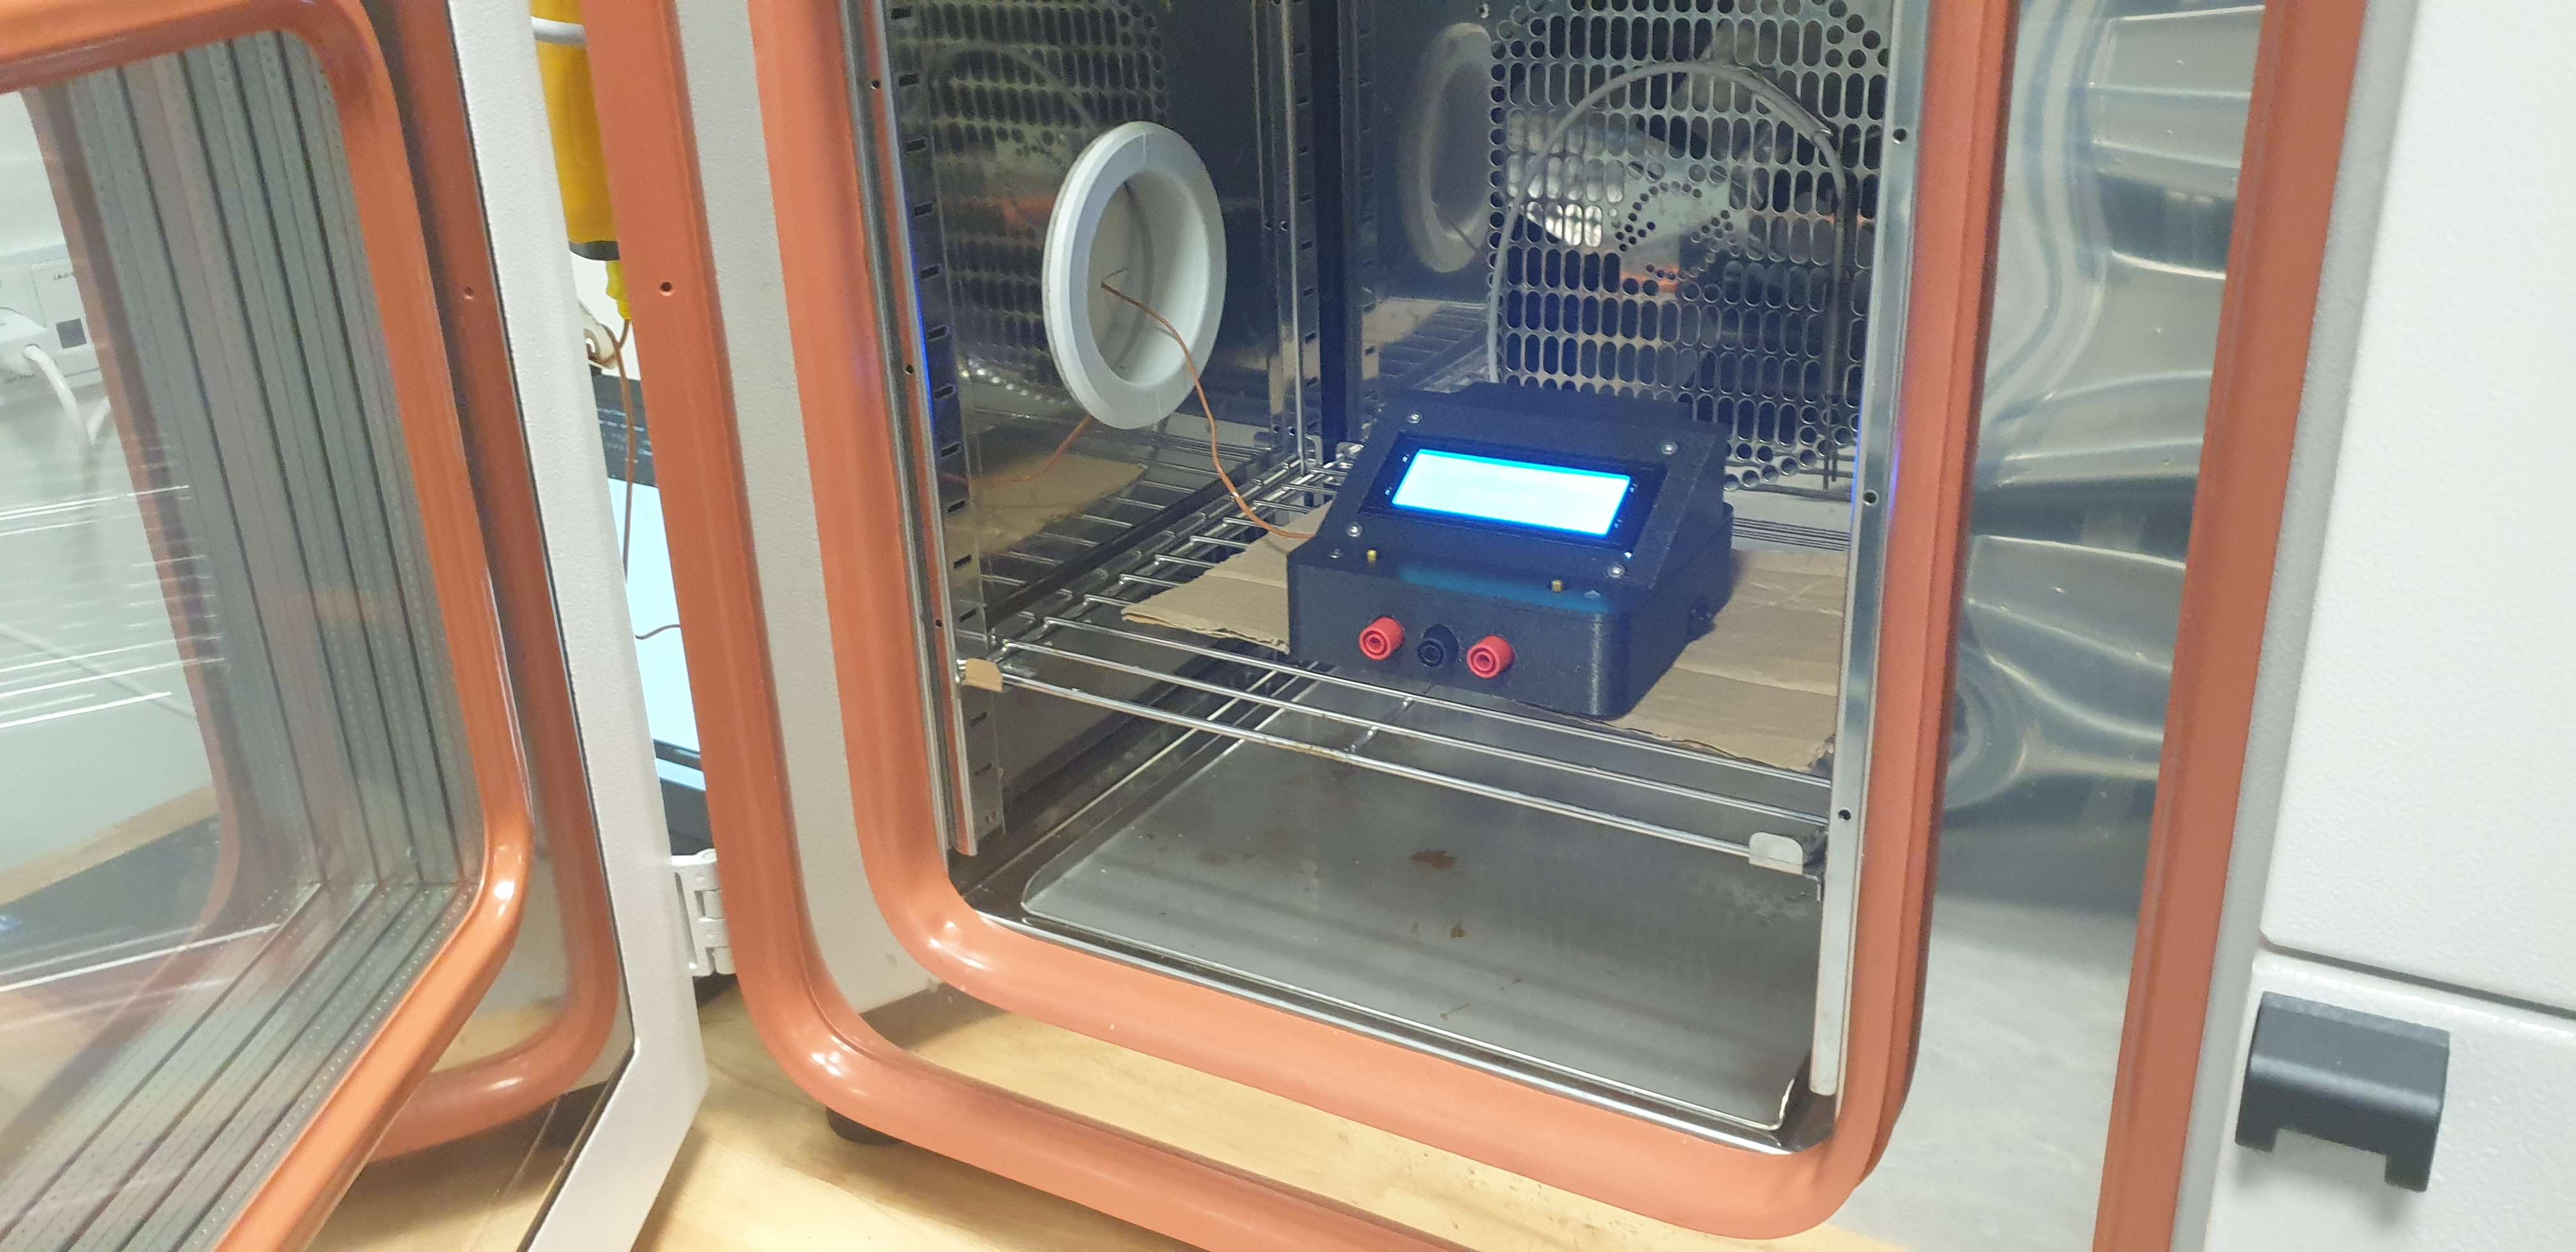
\includegraphics[height=6cm]{images/temp_test_setup.jpg}}
    \caption{Temperature test setup, inside}
    \label{fig:TM1}
\end{figure}

\begin{figure}[h]
    \centering
    \frame{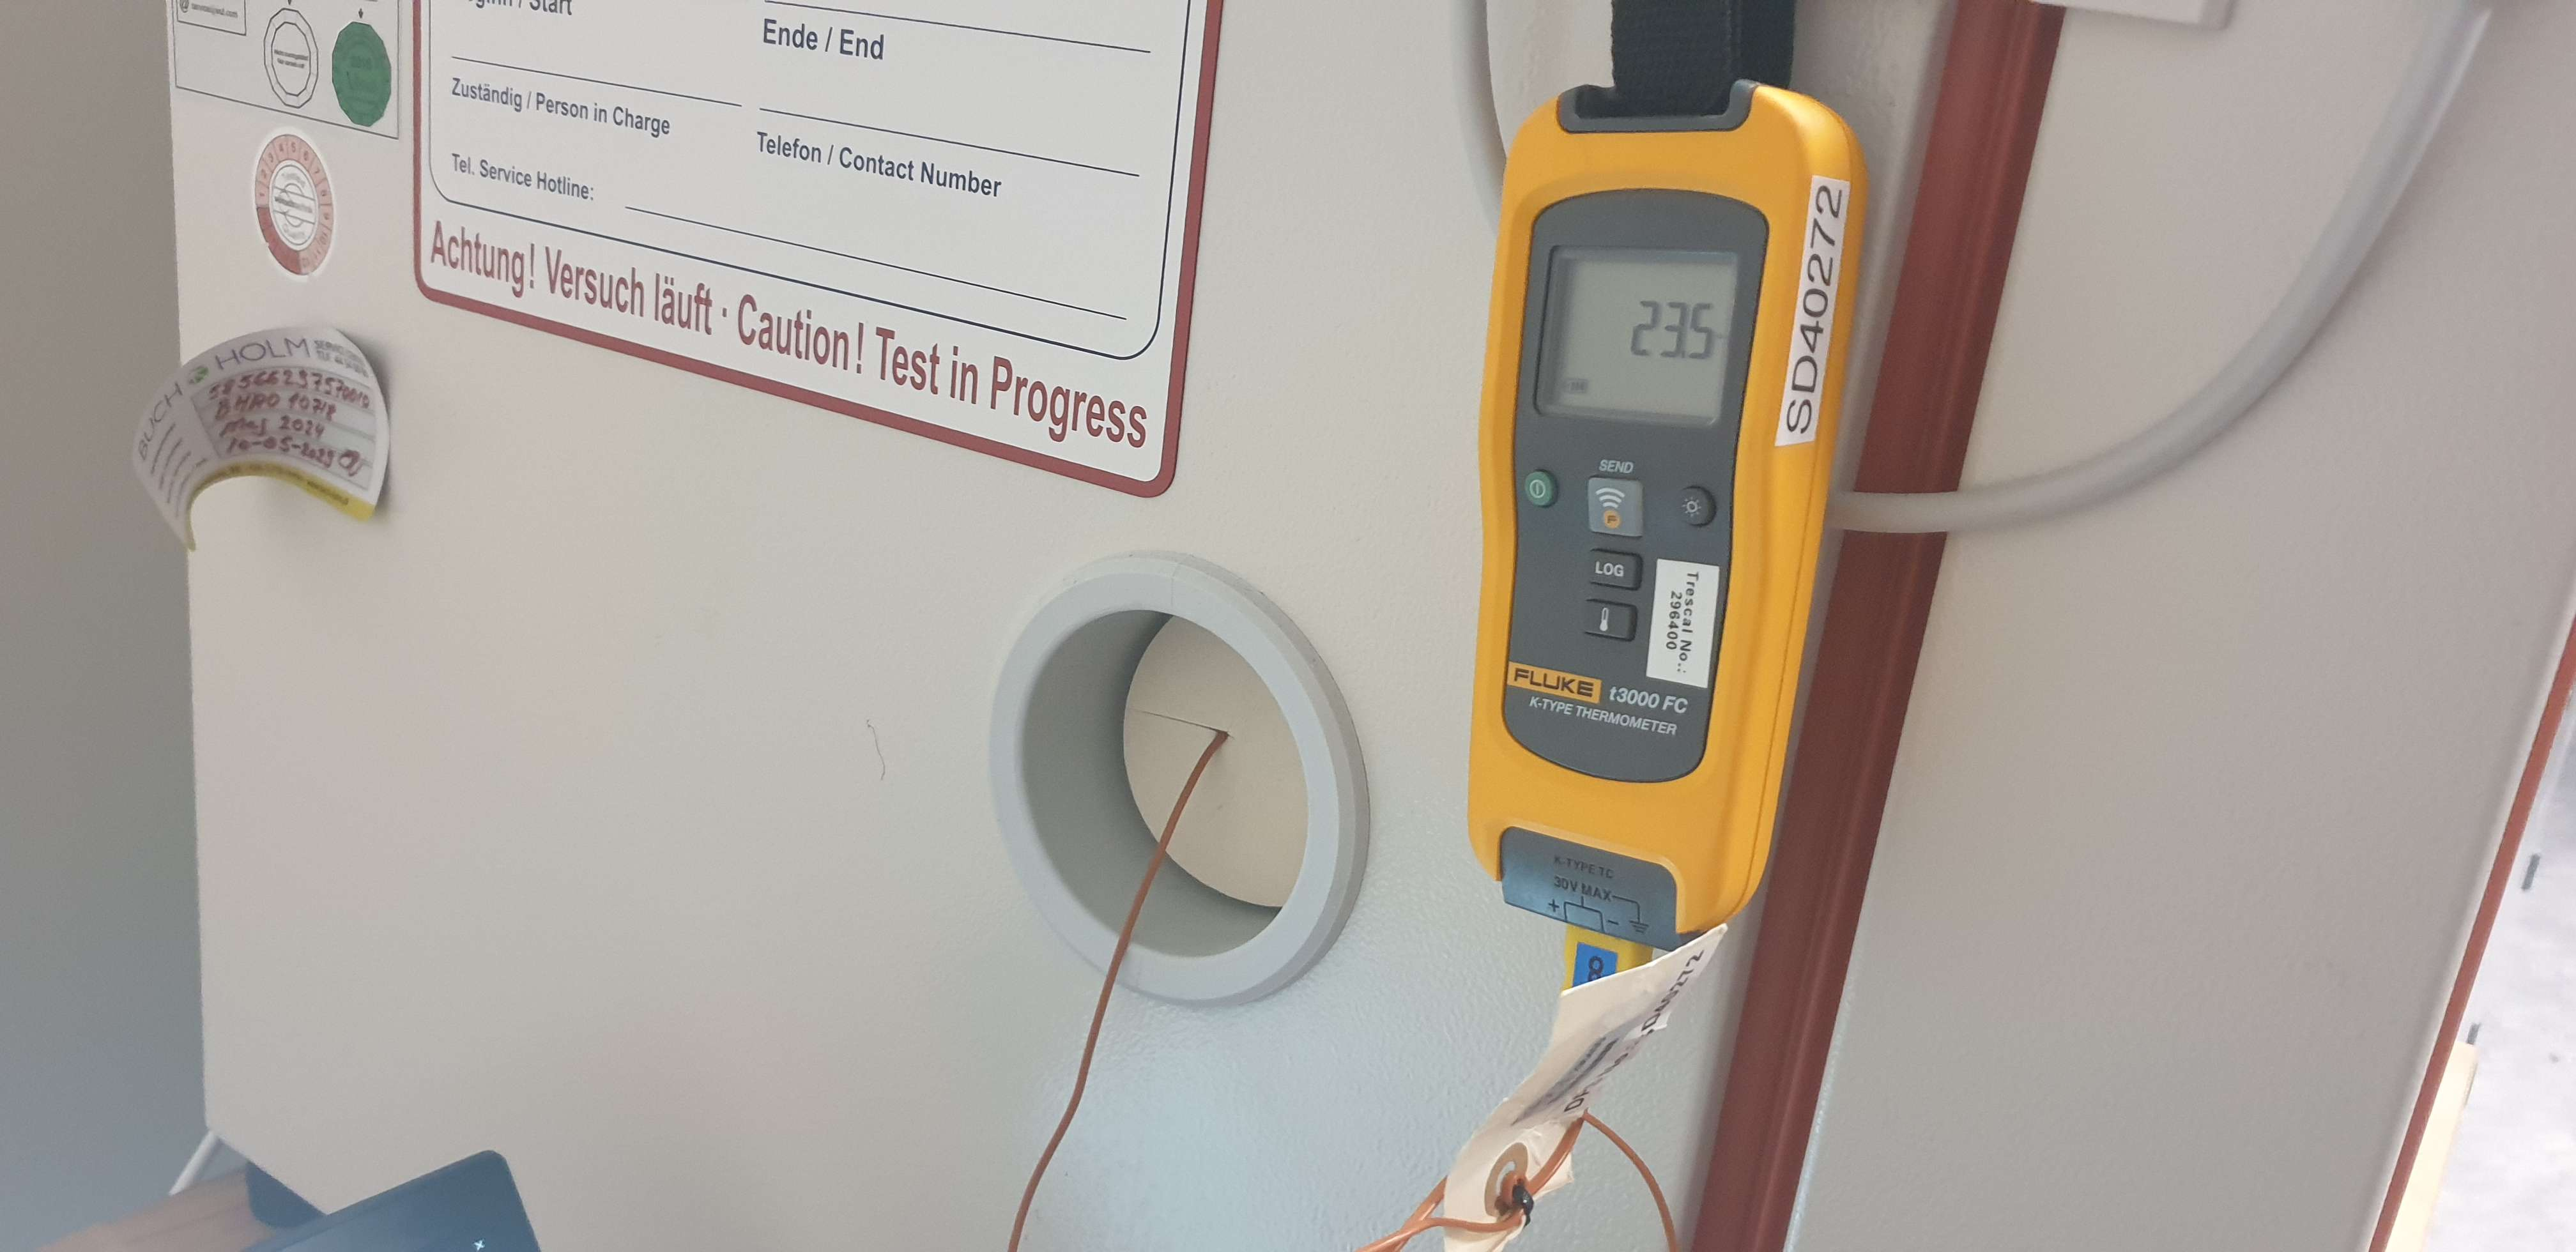
\includegraphics[height=6cm]{images/TSetup2.jpg}}
    \caption{Temperature test setup, outside}
    \label{fig:TM2}
\end{figure}

\begin{figure}[h]
    \centering
    \frame{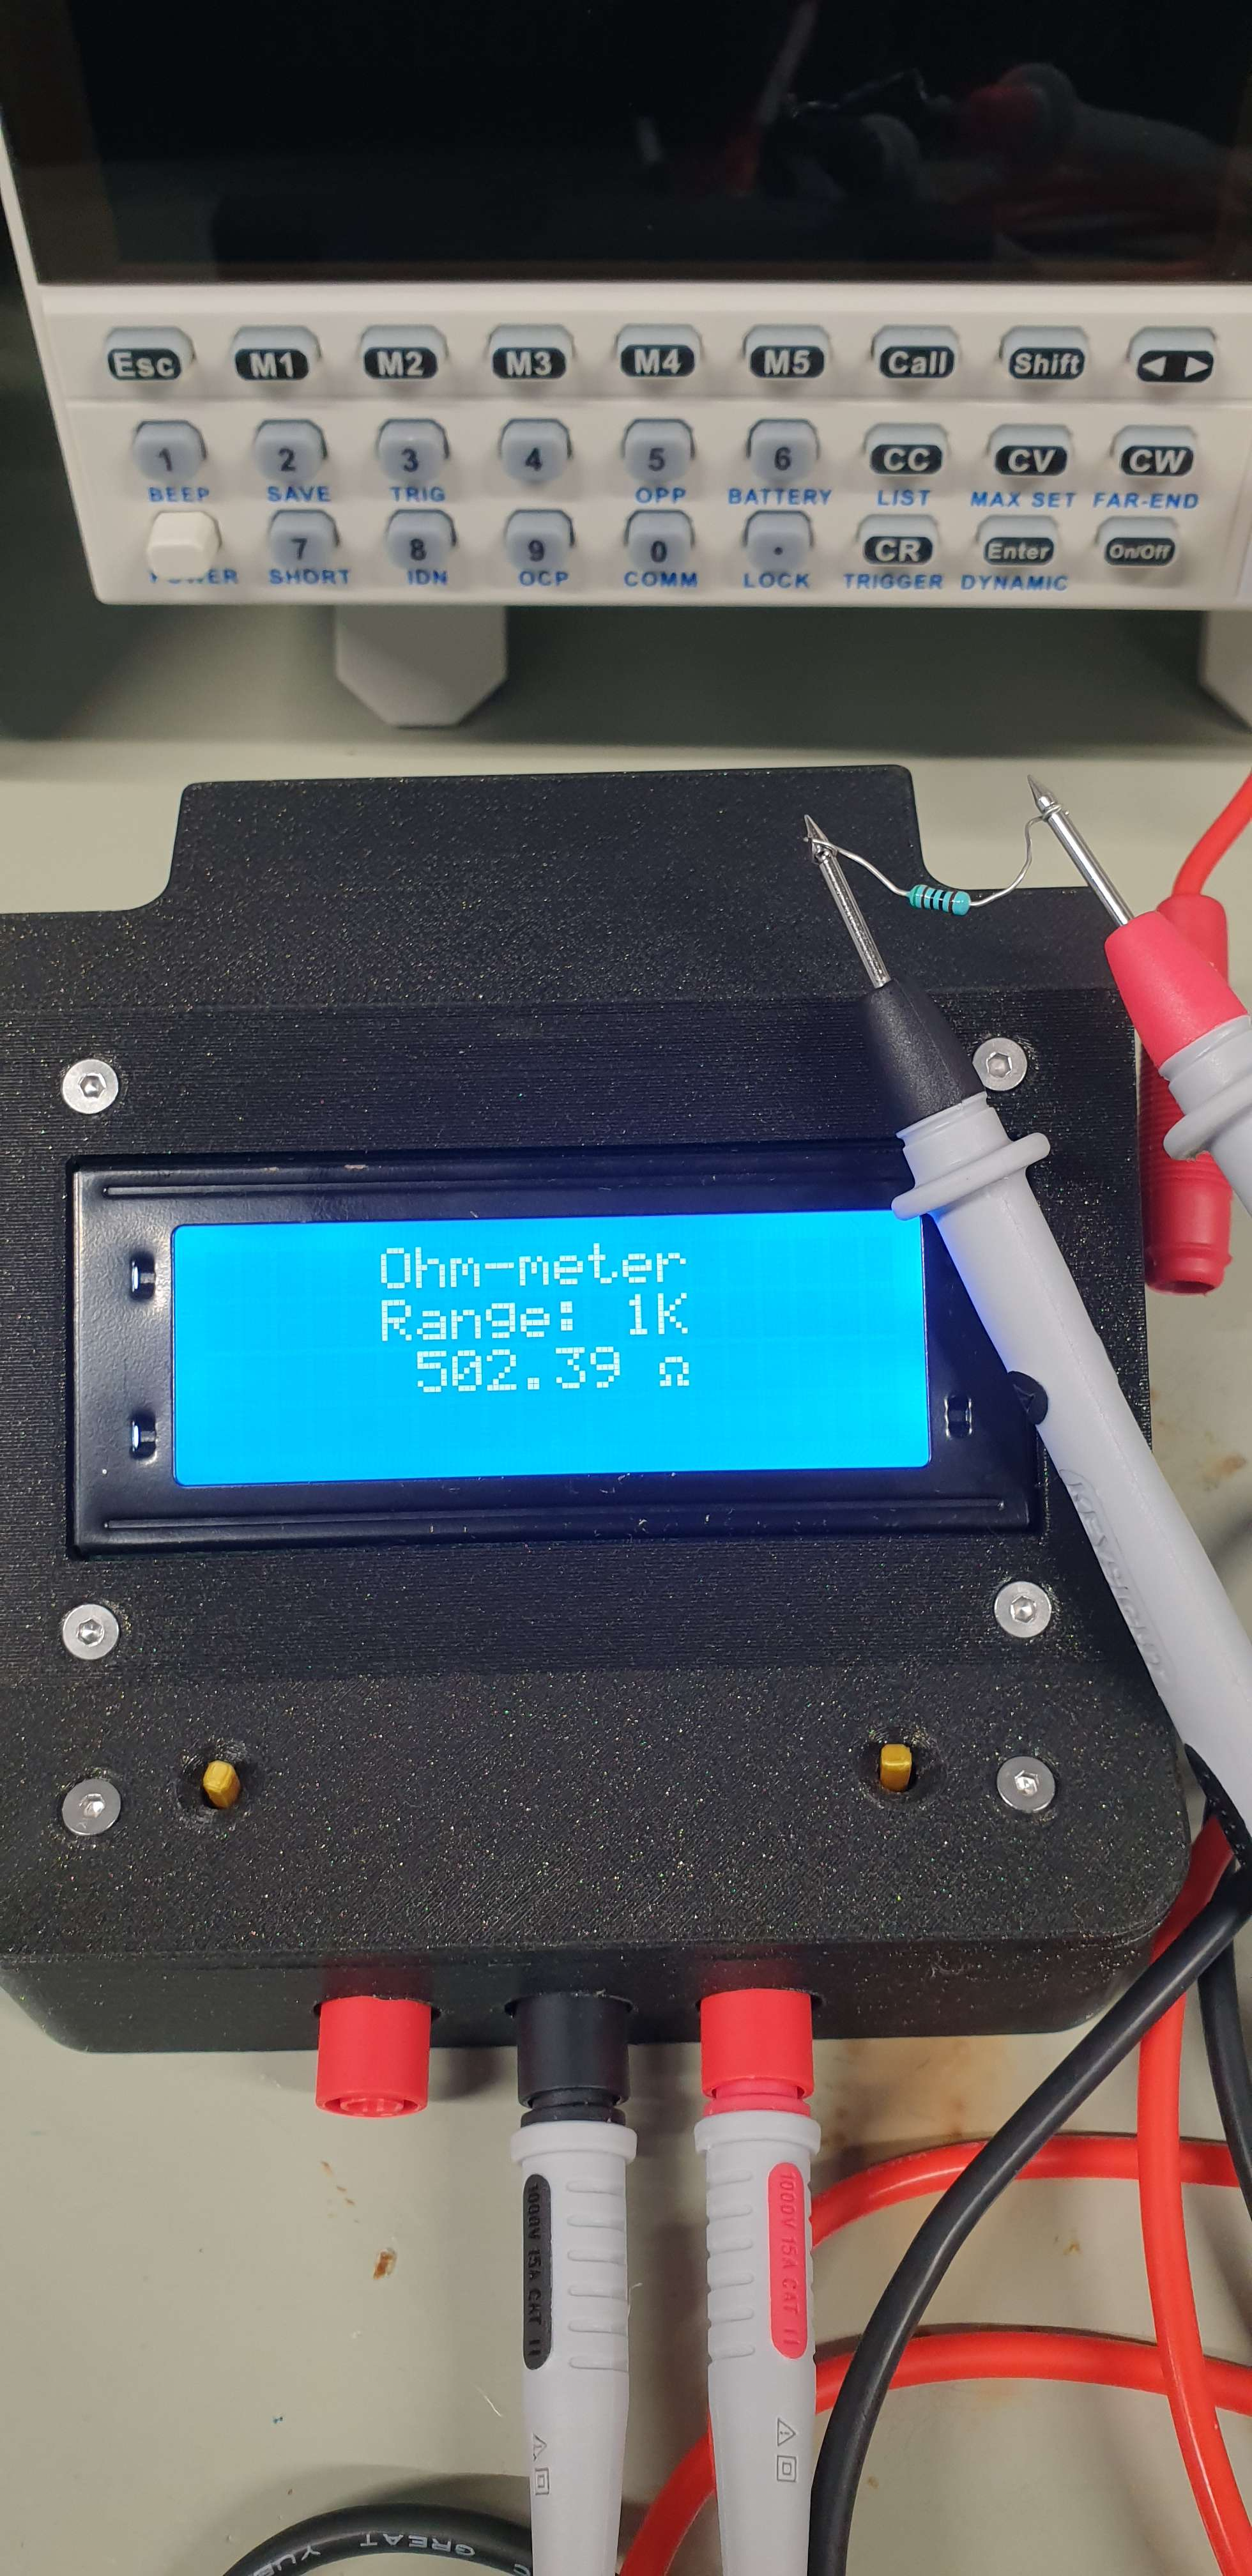
\includegraphics[height=7cm]{images//Measure/resMeas.jpg}}
    \caption{Resistance test setup, 510$\Omega$}
    \label{fig:RM1}
\end{figure}

\begin{figure}[h]
    \centering
    \frame{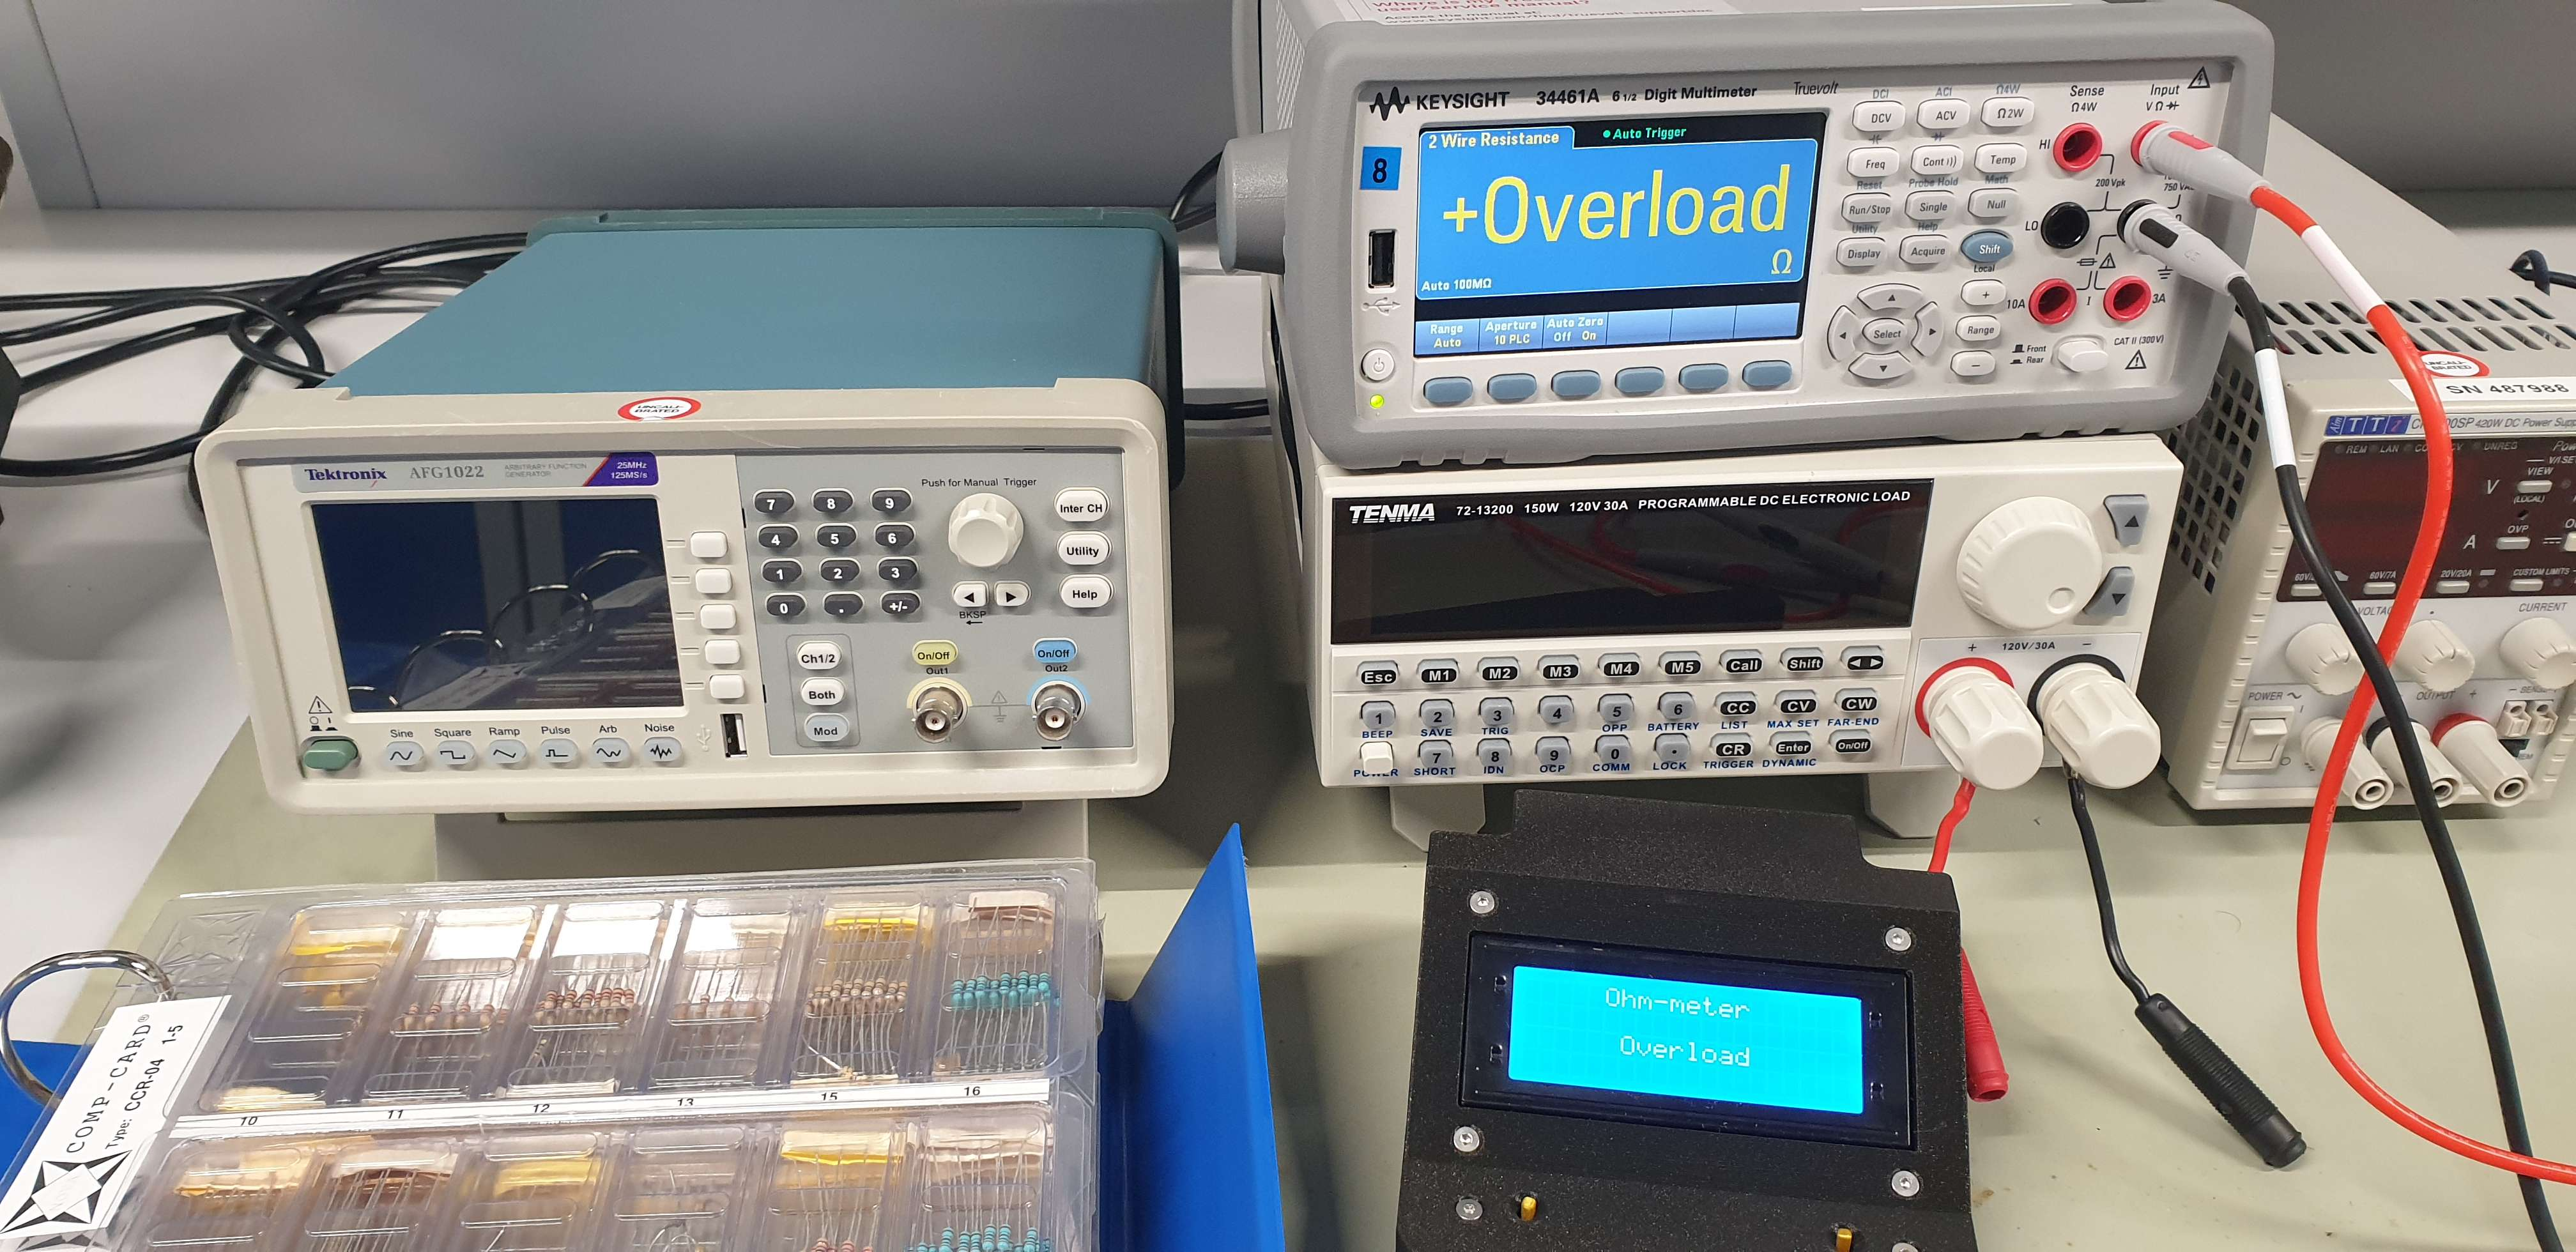
\includegraphics[height=5cm]{images//Measure/resMeas1.jpg}}
    \caption{Resistance test setup, with resistor assortment}
    \label{fig:RM2}
\end{figure}

\begin{figure}[h]
    \centering
    \frame{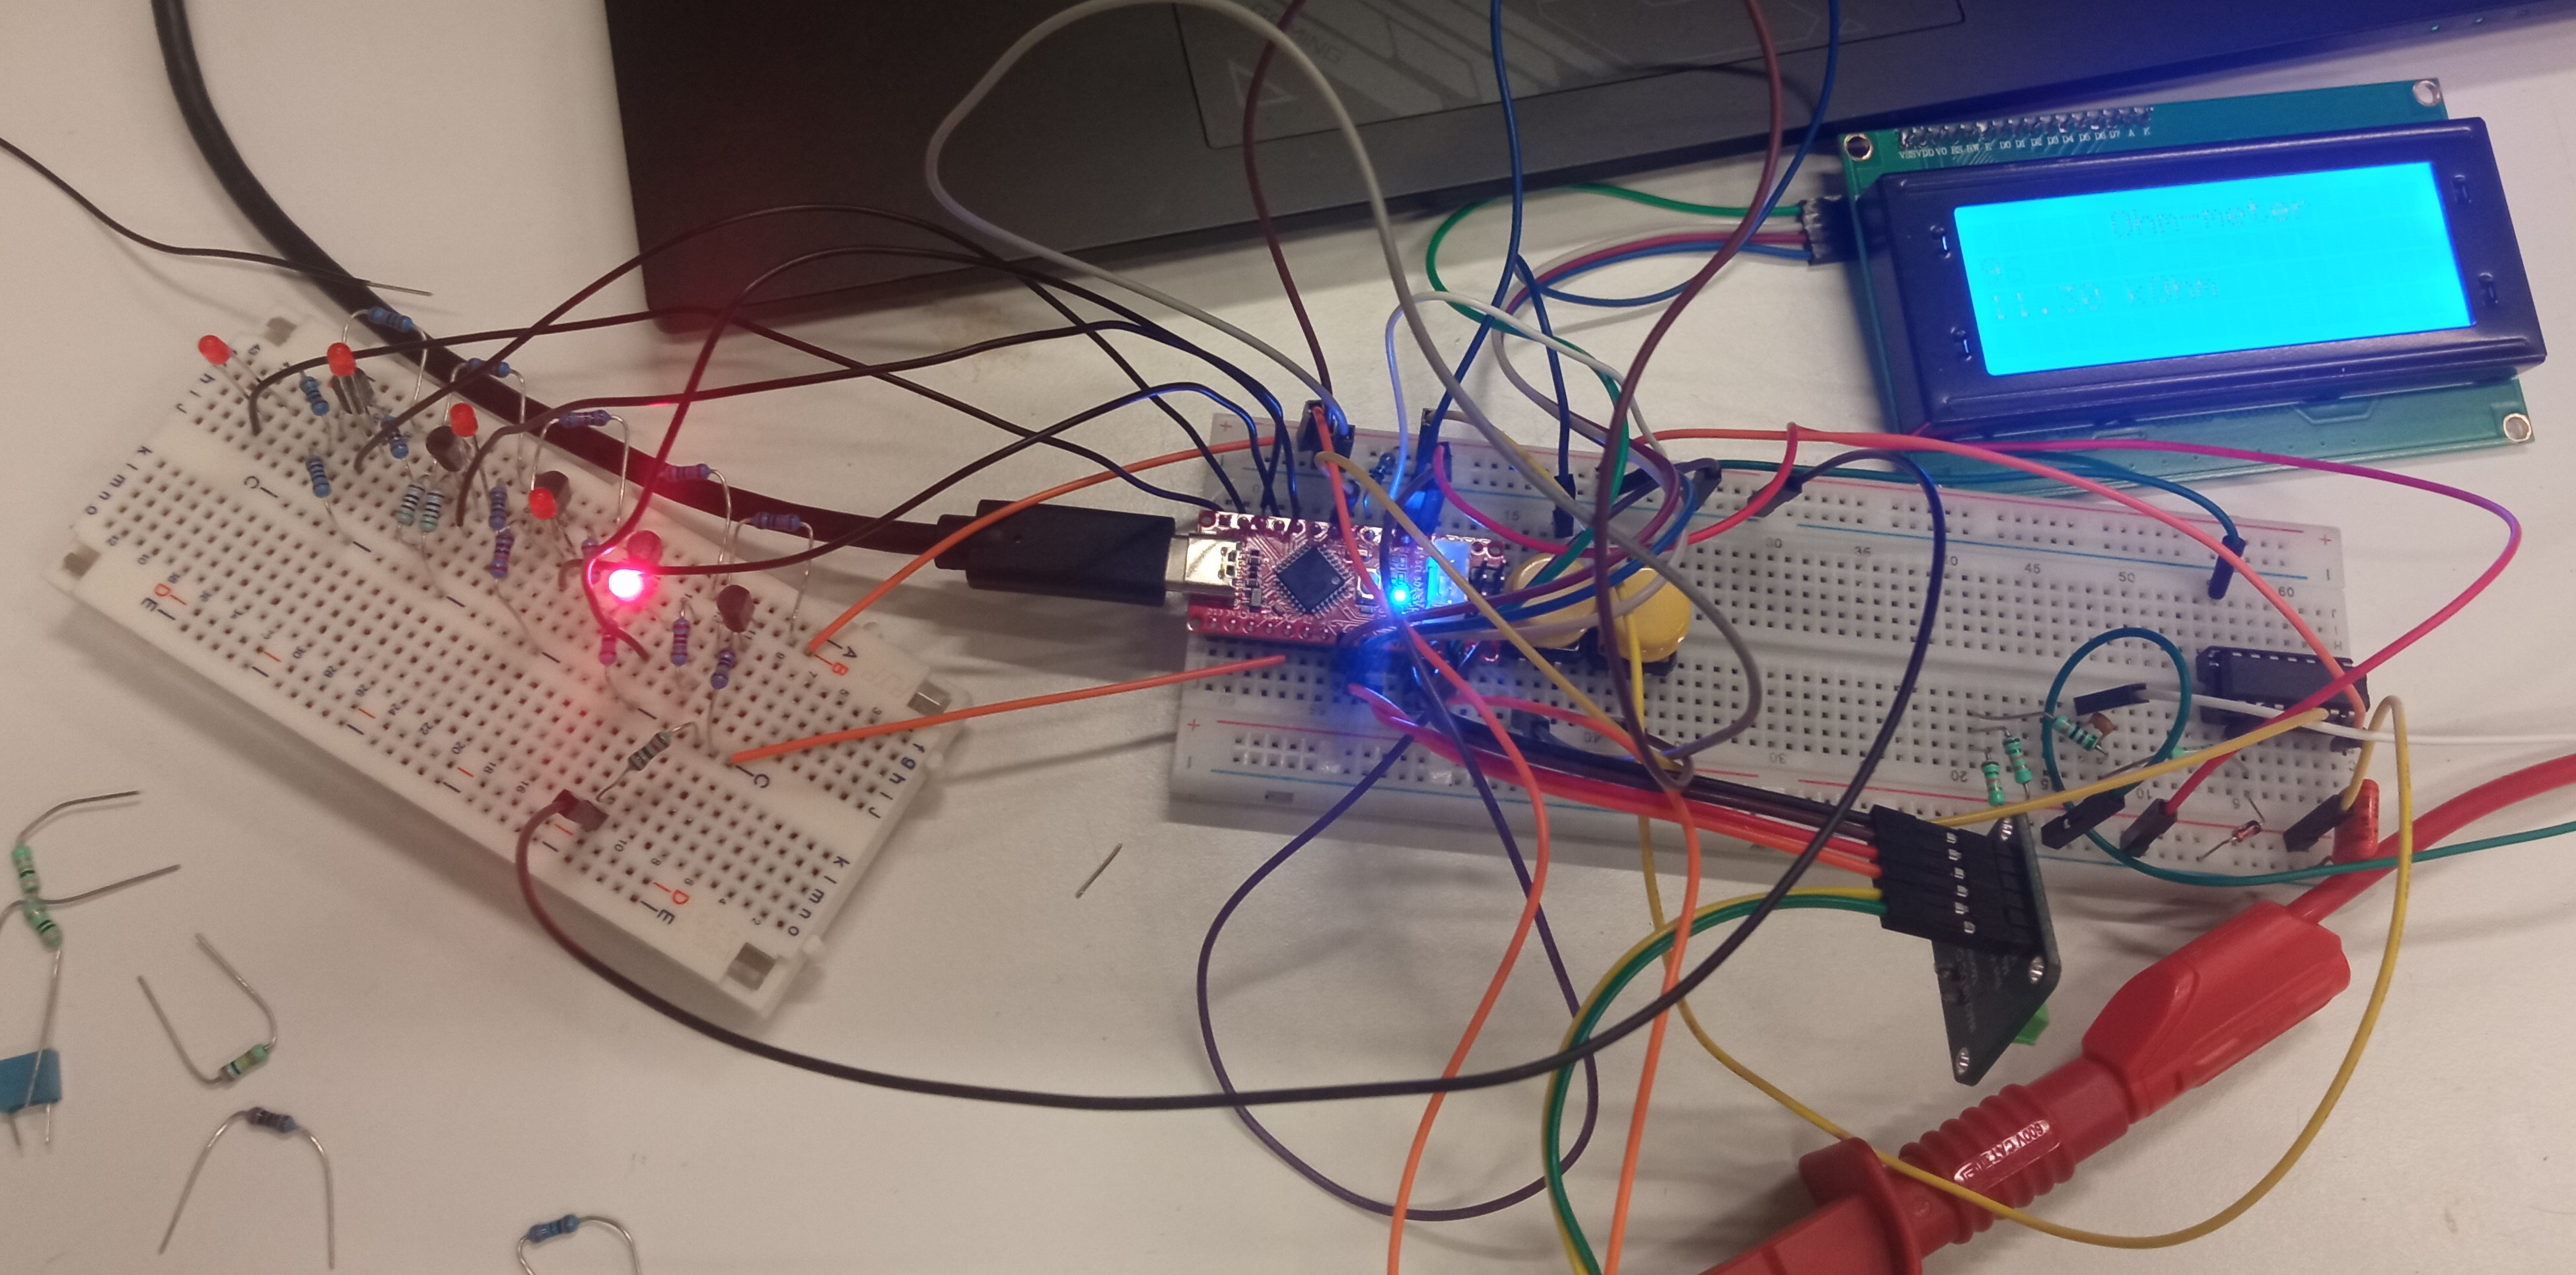
\includegraphics[height=6cm]{images/breadboard_proto.jpg}}
    \caption{Breadboard prototyping}
    \label{fig:breadboardPrototyping}
\end{figure}

\begin{figure}[h]
    \centering
    \frame{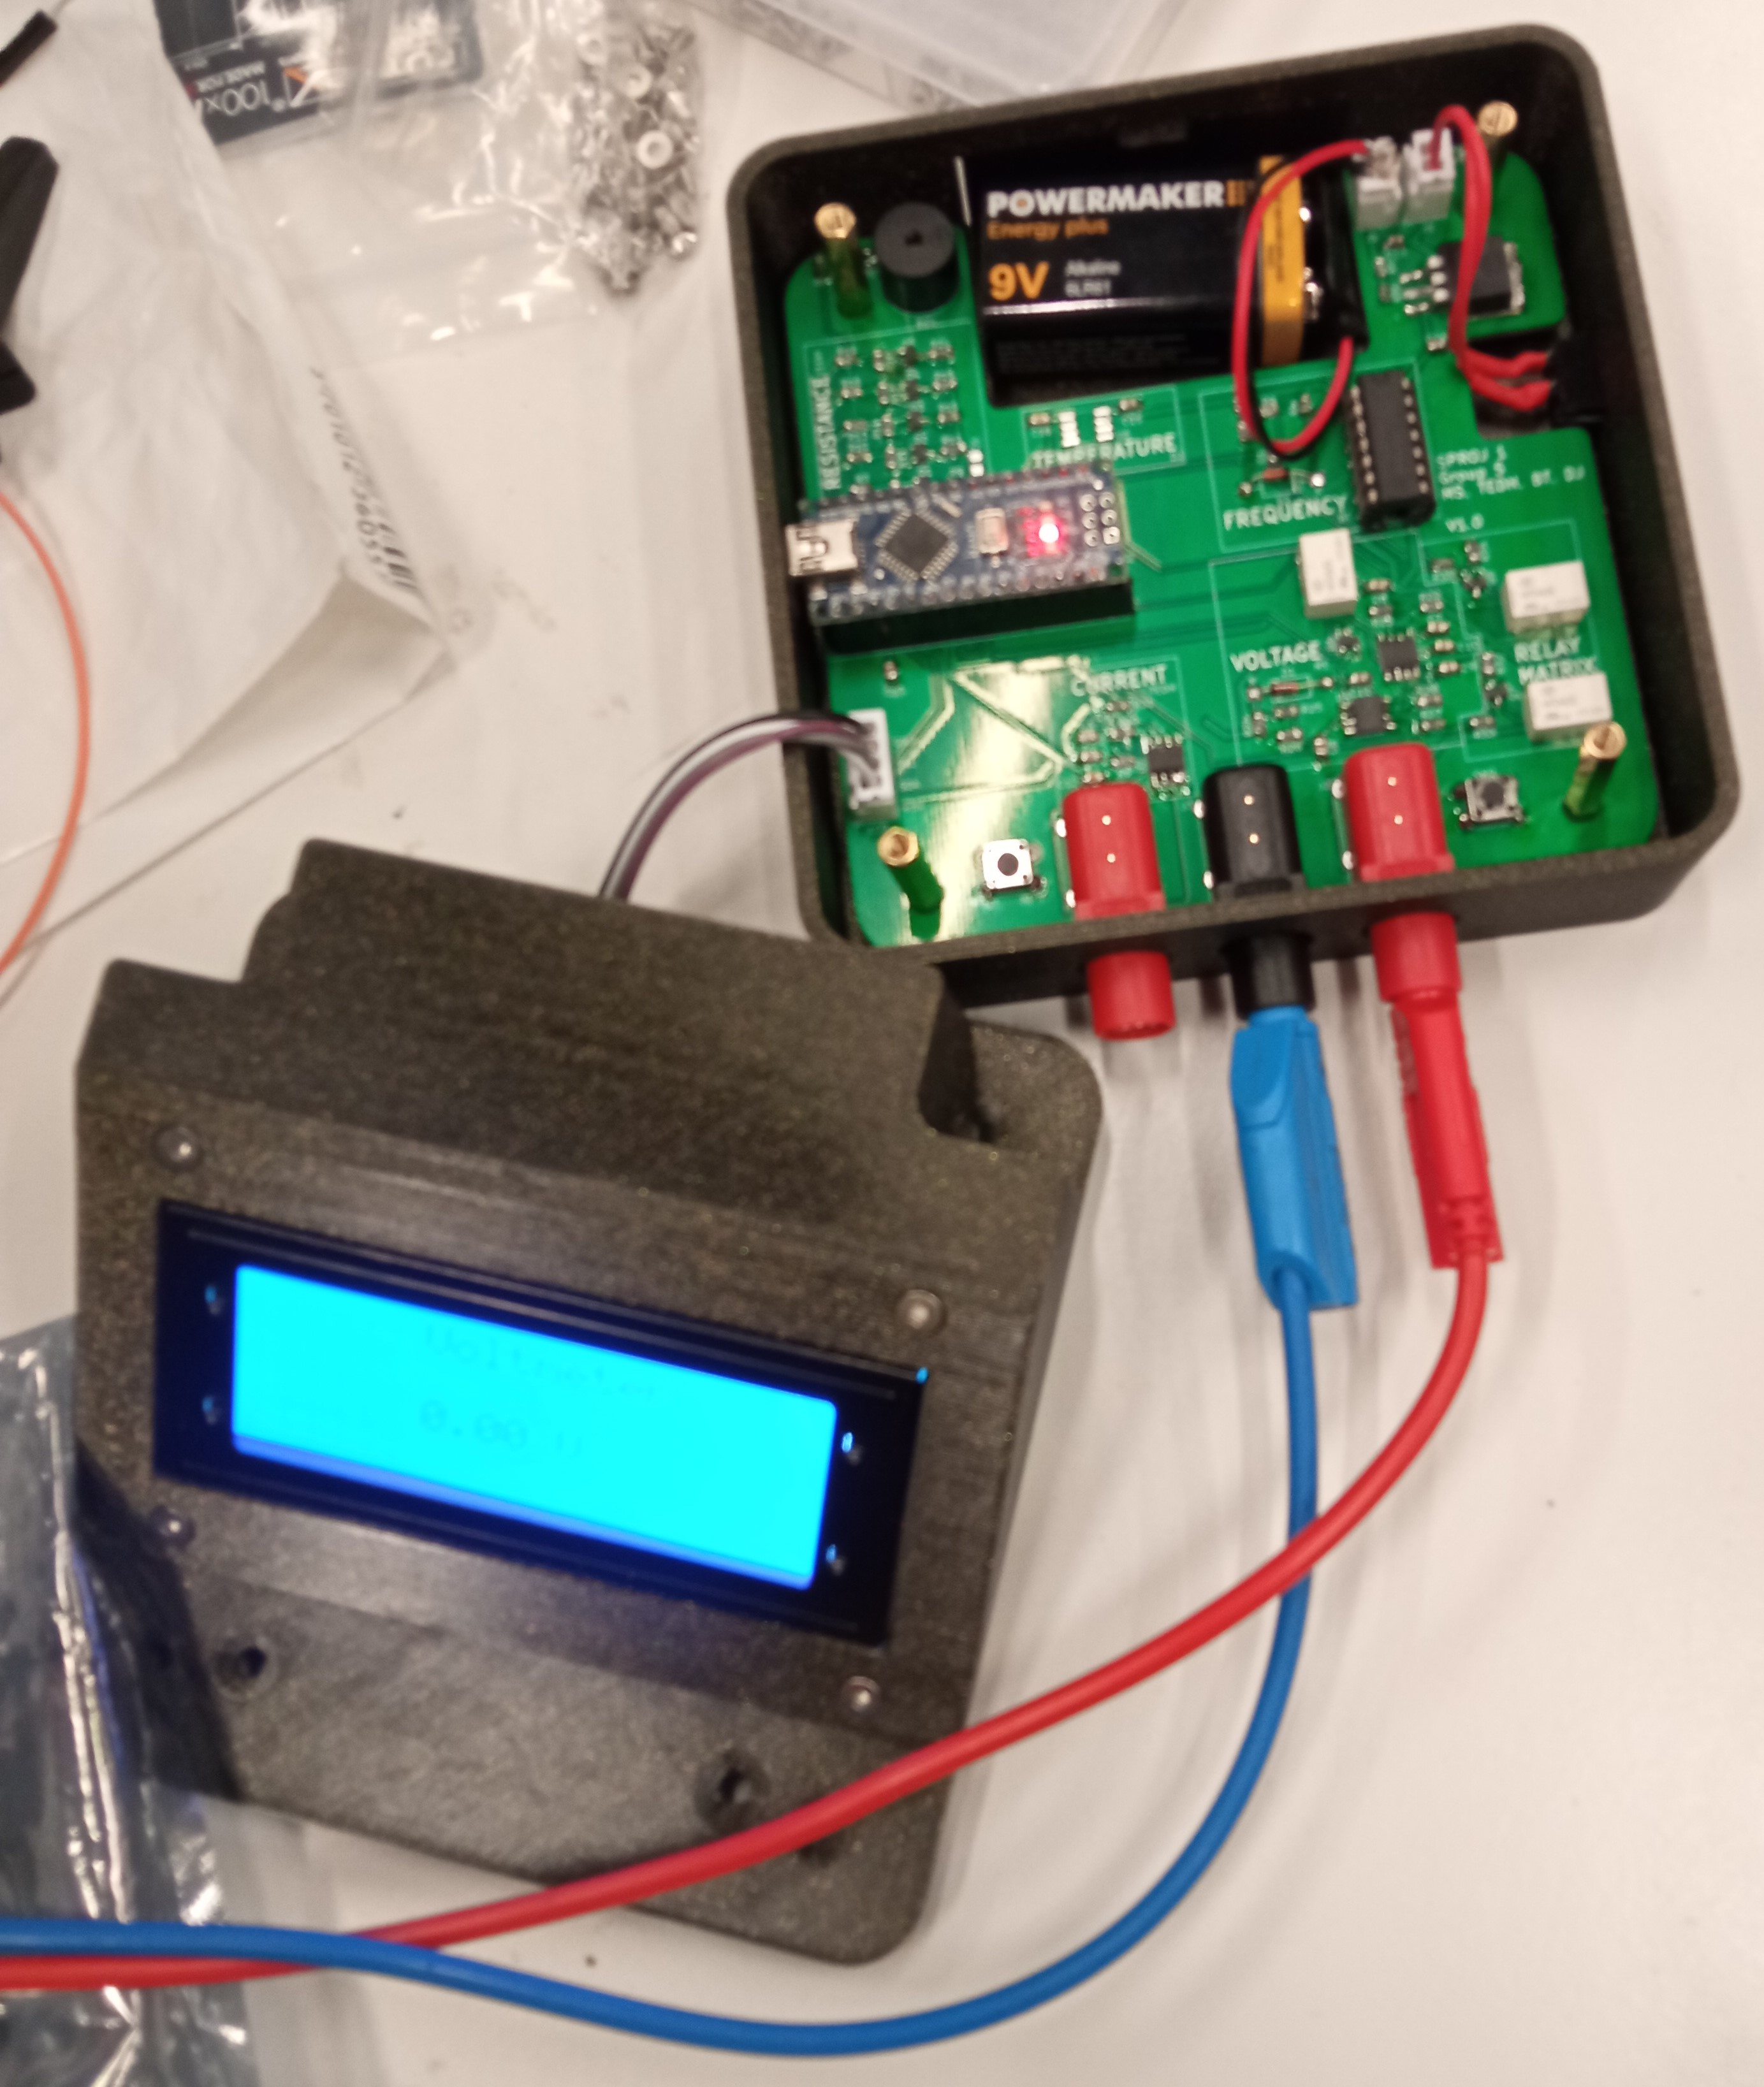
\includegraphics[height=8cm]{images/MM_V1.jpg}}
    \caption{Multimeter V1.0 during testing}
    \label{fig:MMV1}
\end{figure}

\begin{figure}[h]
    \centering
    \frame{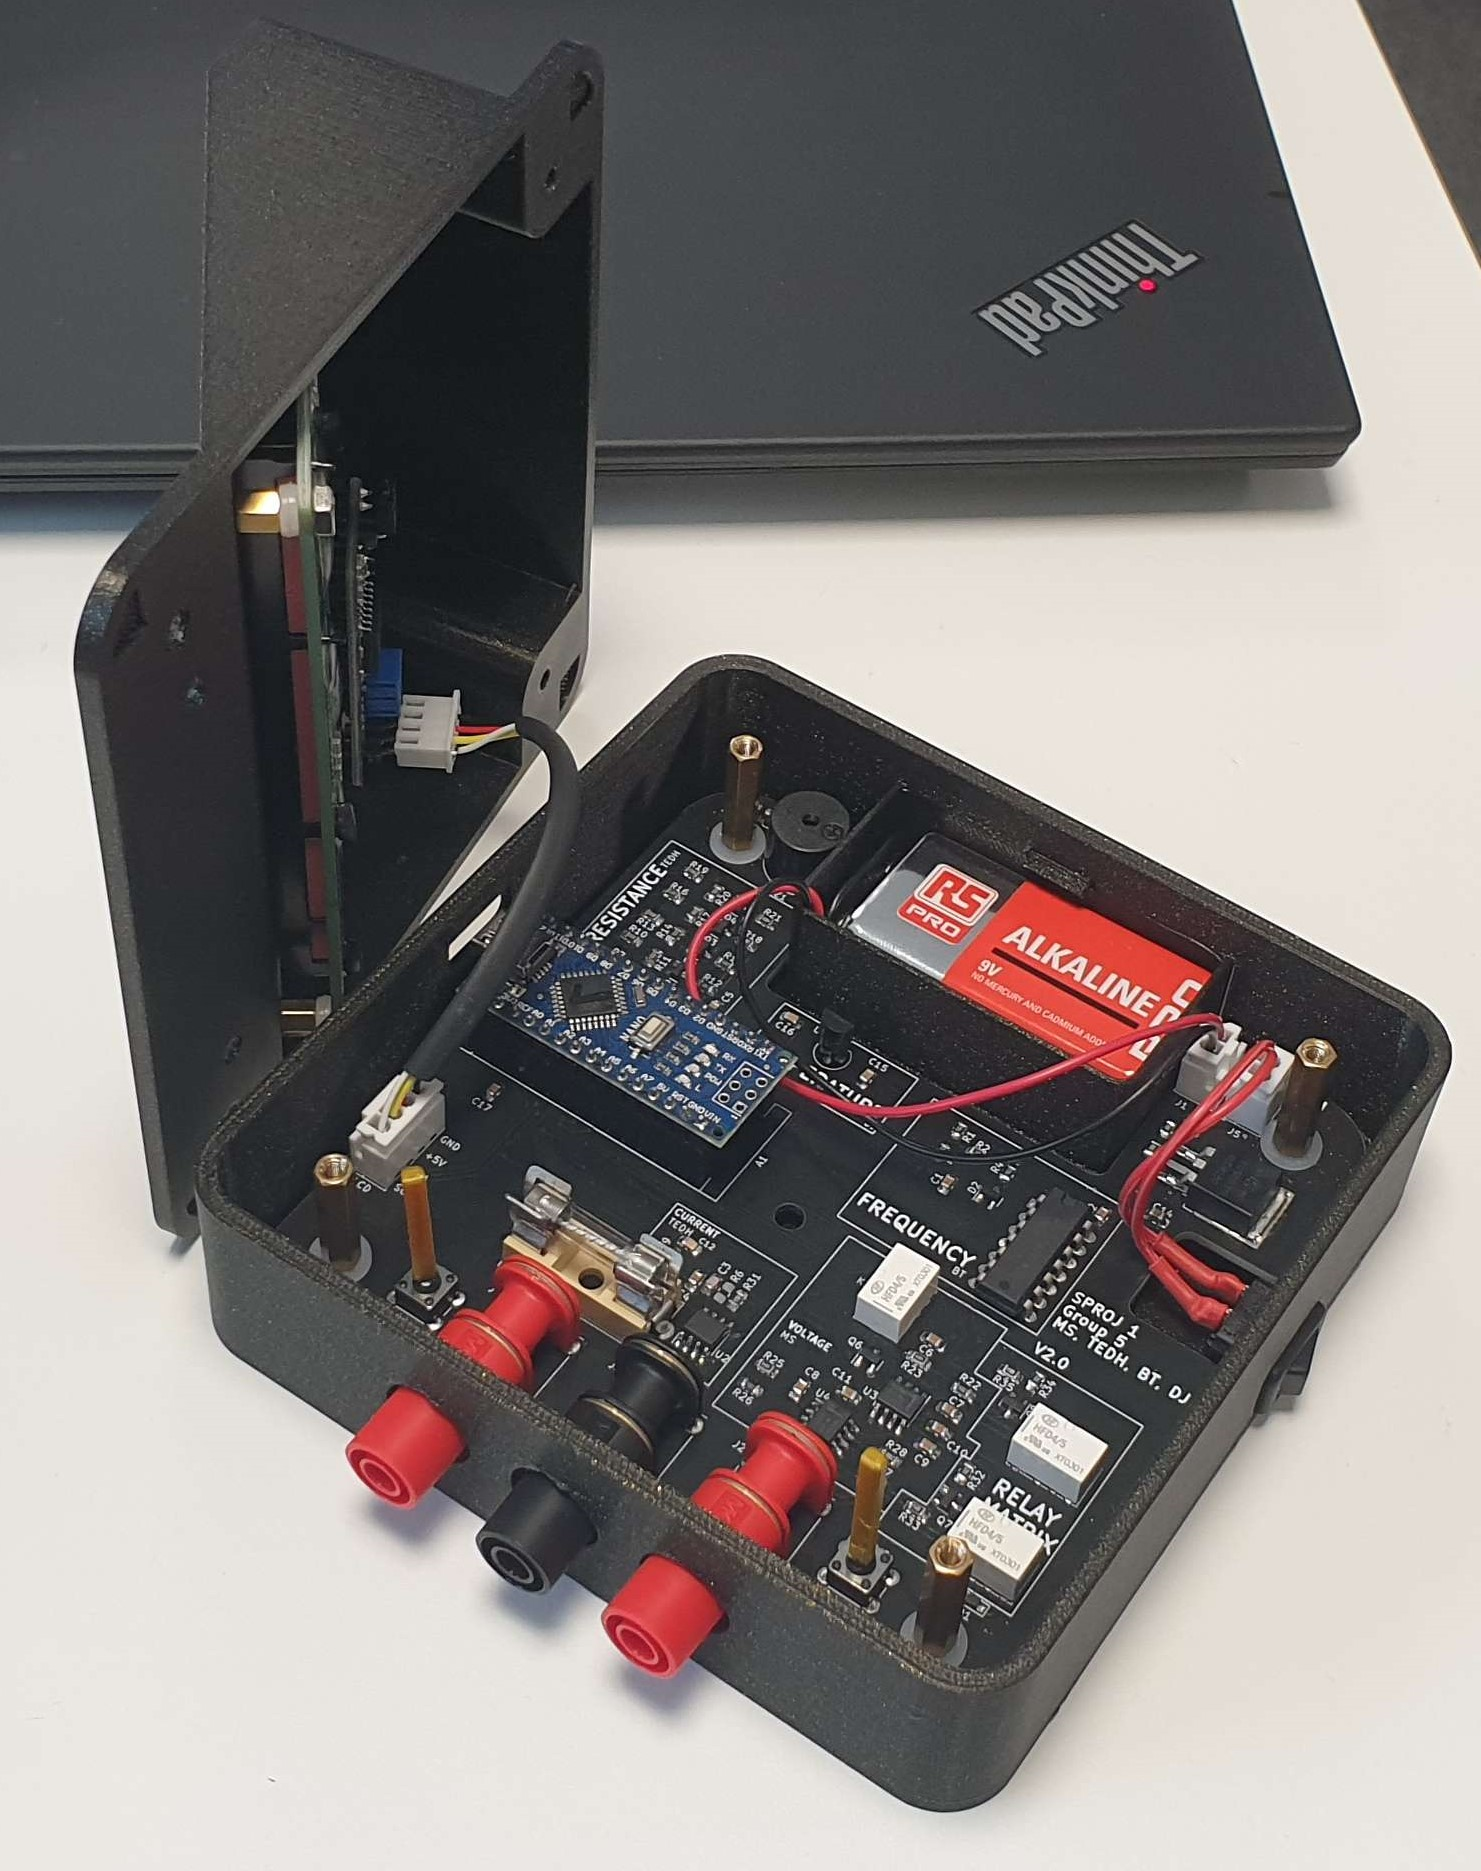
\includegraphics[height=8cm]{images/MM_Final.jpg}}
    \caption{Multimeter, final iteration}
    \label{fig:MM_final}
\end{figure}

\begin{figure}[h]
    \centering
    \frame{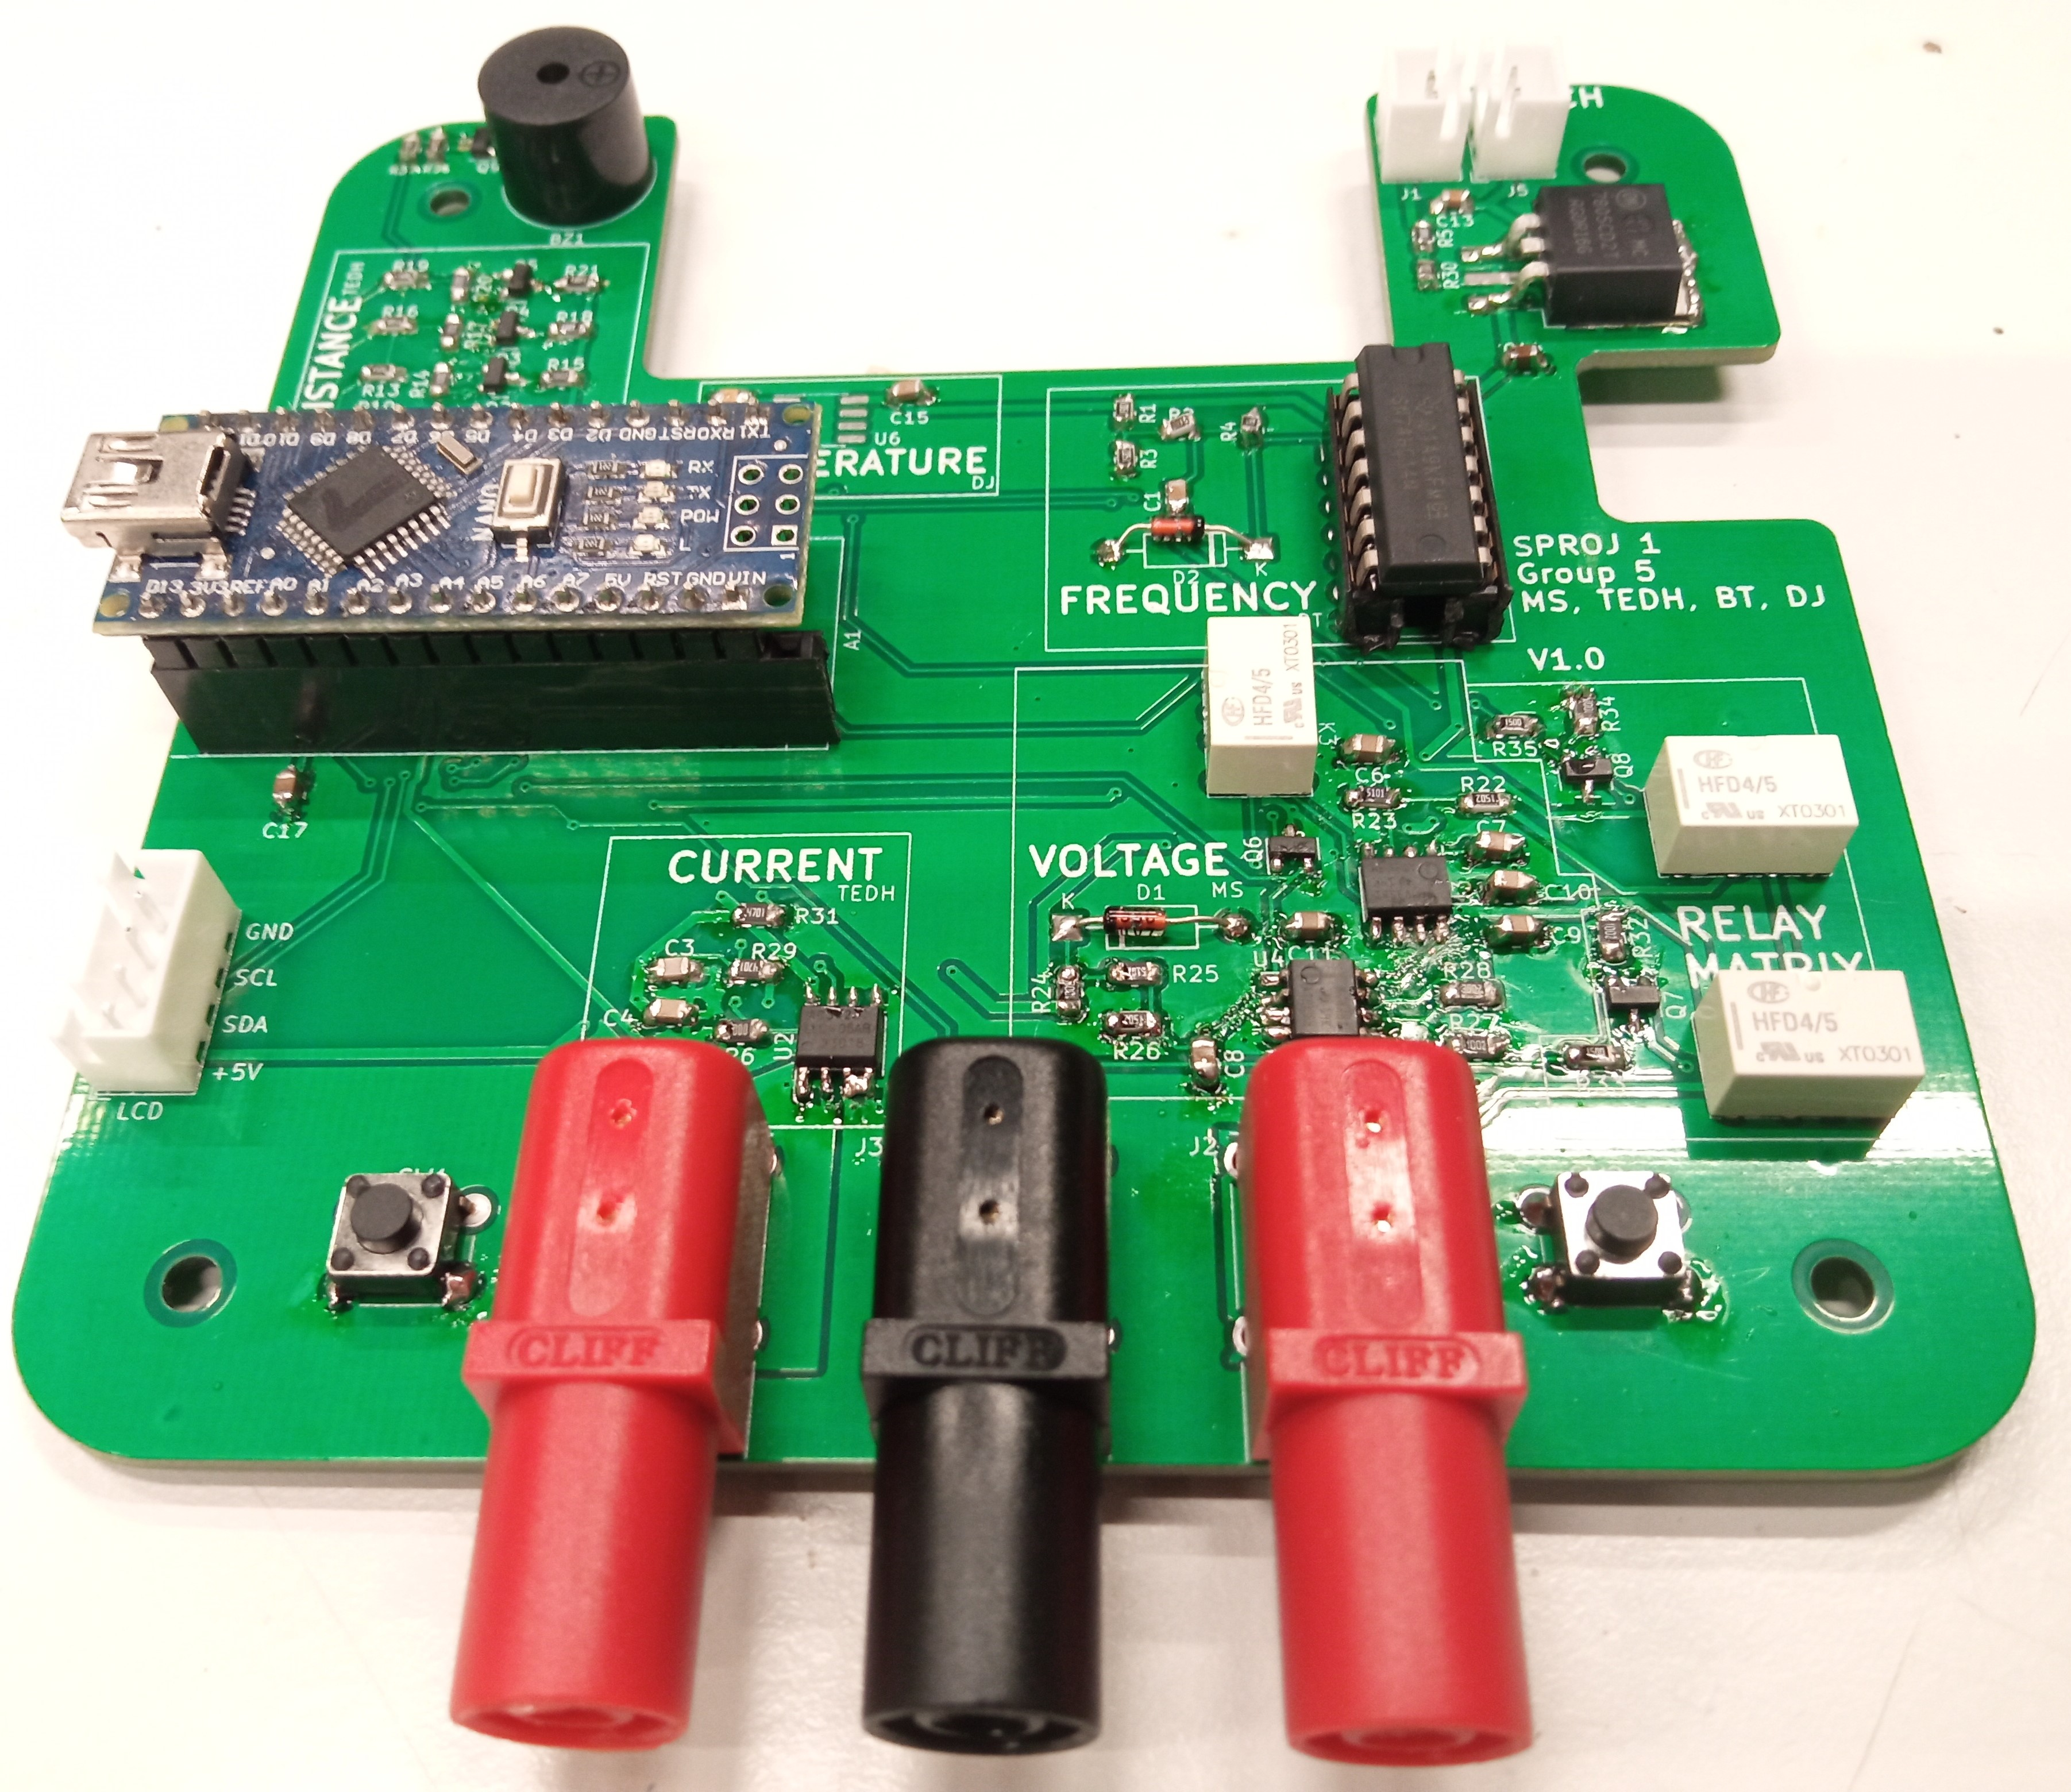
\includegraphics[height=7cm]{images/pcb_v1.jpg}}
    \caption{PCB Version V1.0}
    \label{fig:pcbV1}
\end{figure}

\begin{figure}[h]
    \centering
    \frame{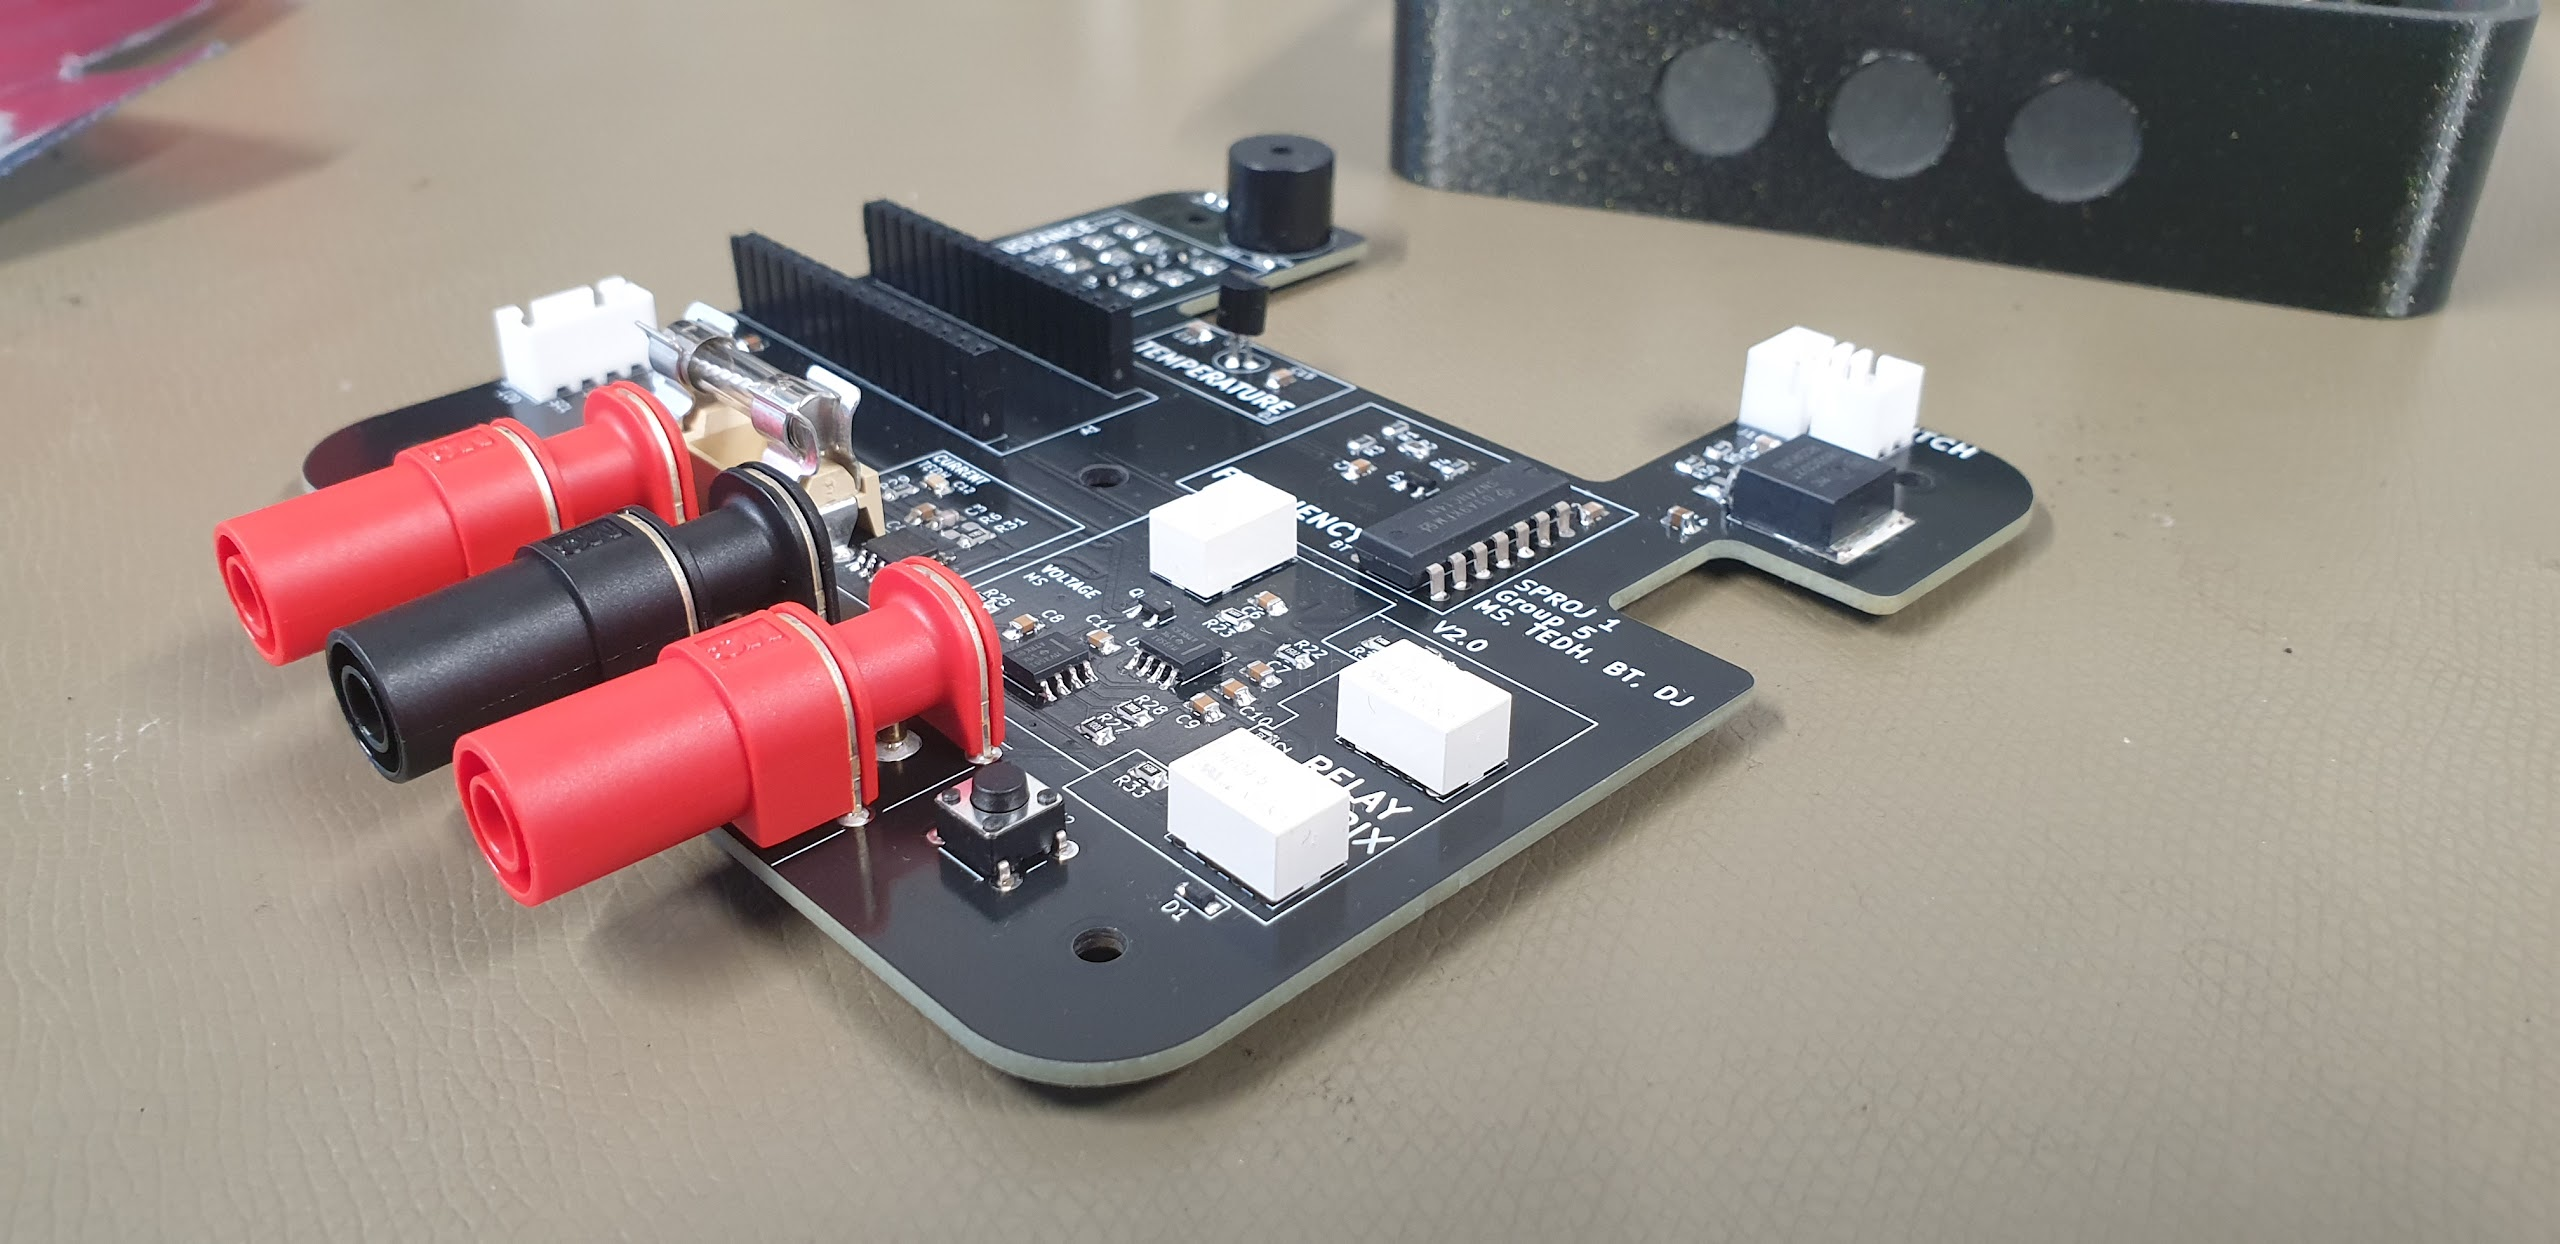
\includegraphics[width=1\linewidth]{images/PCB2.0V.jpg}}
    \caption{PCB Version V2.0}
    \label{fig:pcbV1}
\end{figure}

\begin{figure}[h]
    \centering
    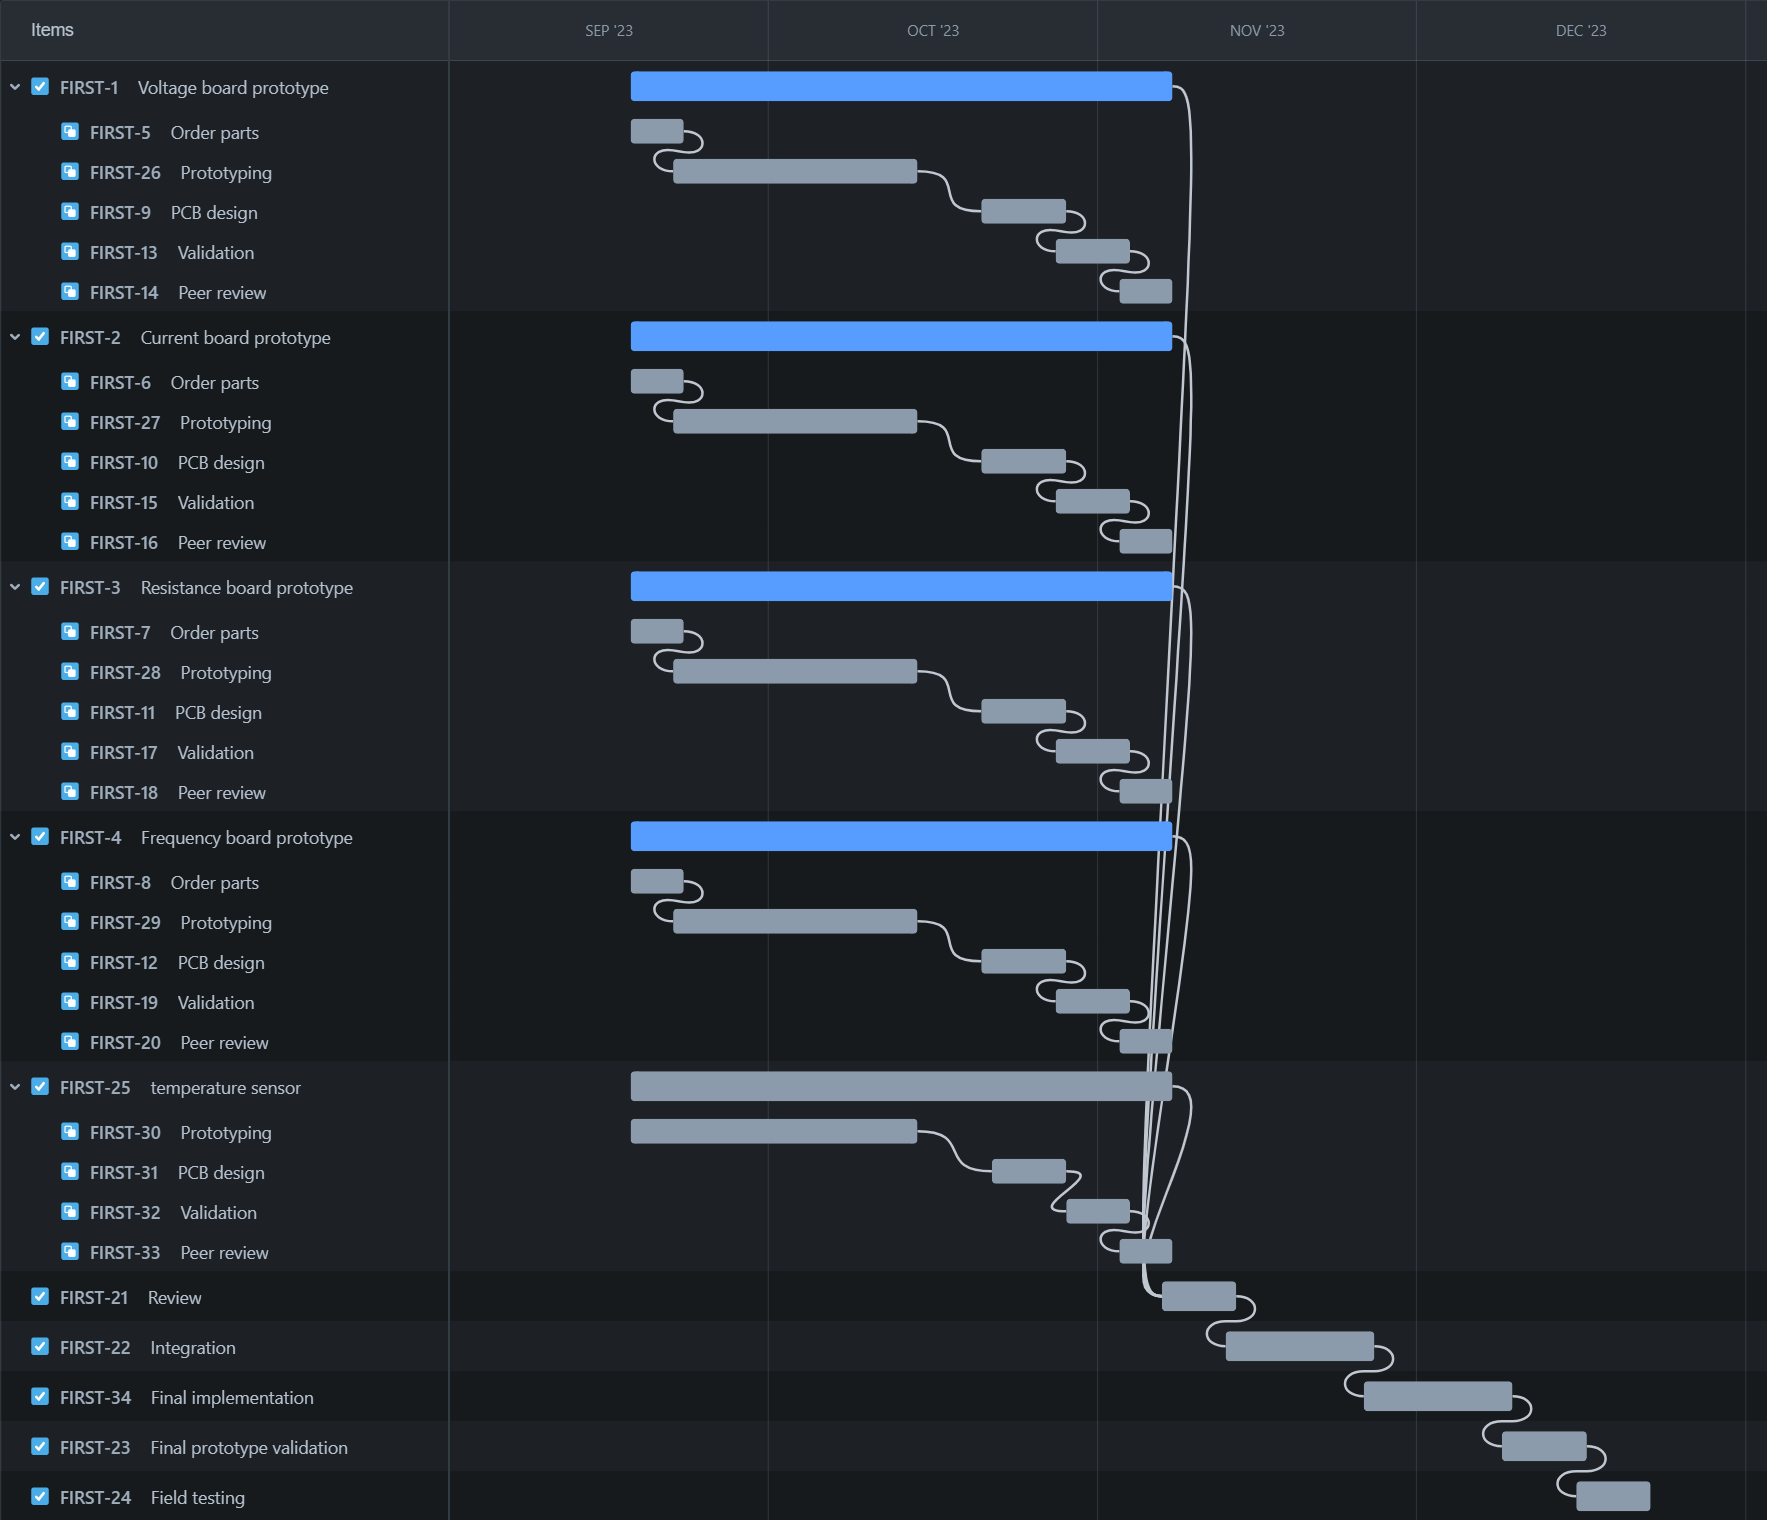
\includegraphics[width=1\linewidth]{images/SPROJ1G5_Timeline.png}
    \caption{Time plan}
    \label{fig:TP}
\end{figure}

\clearpage

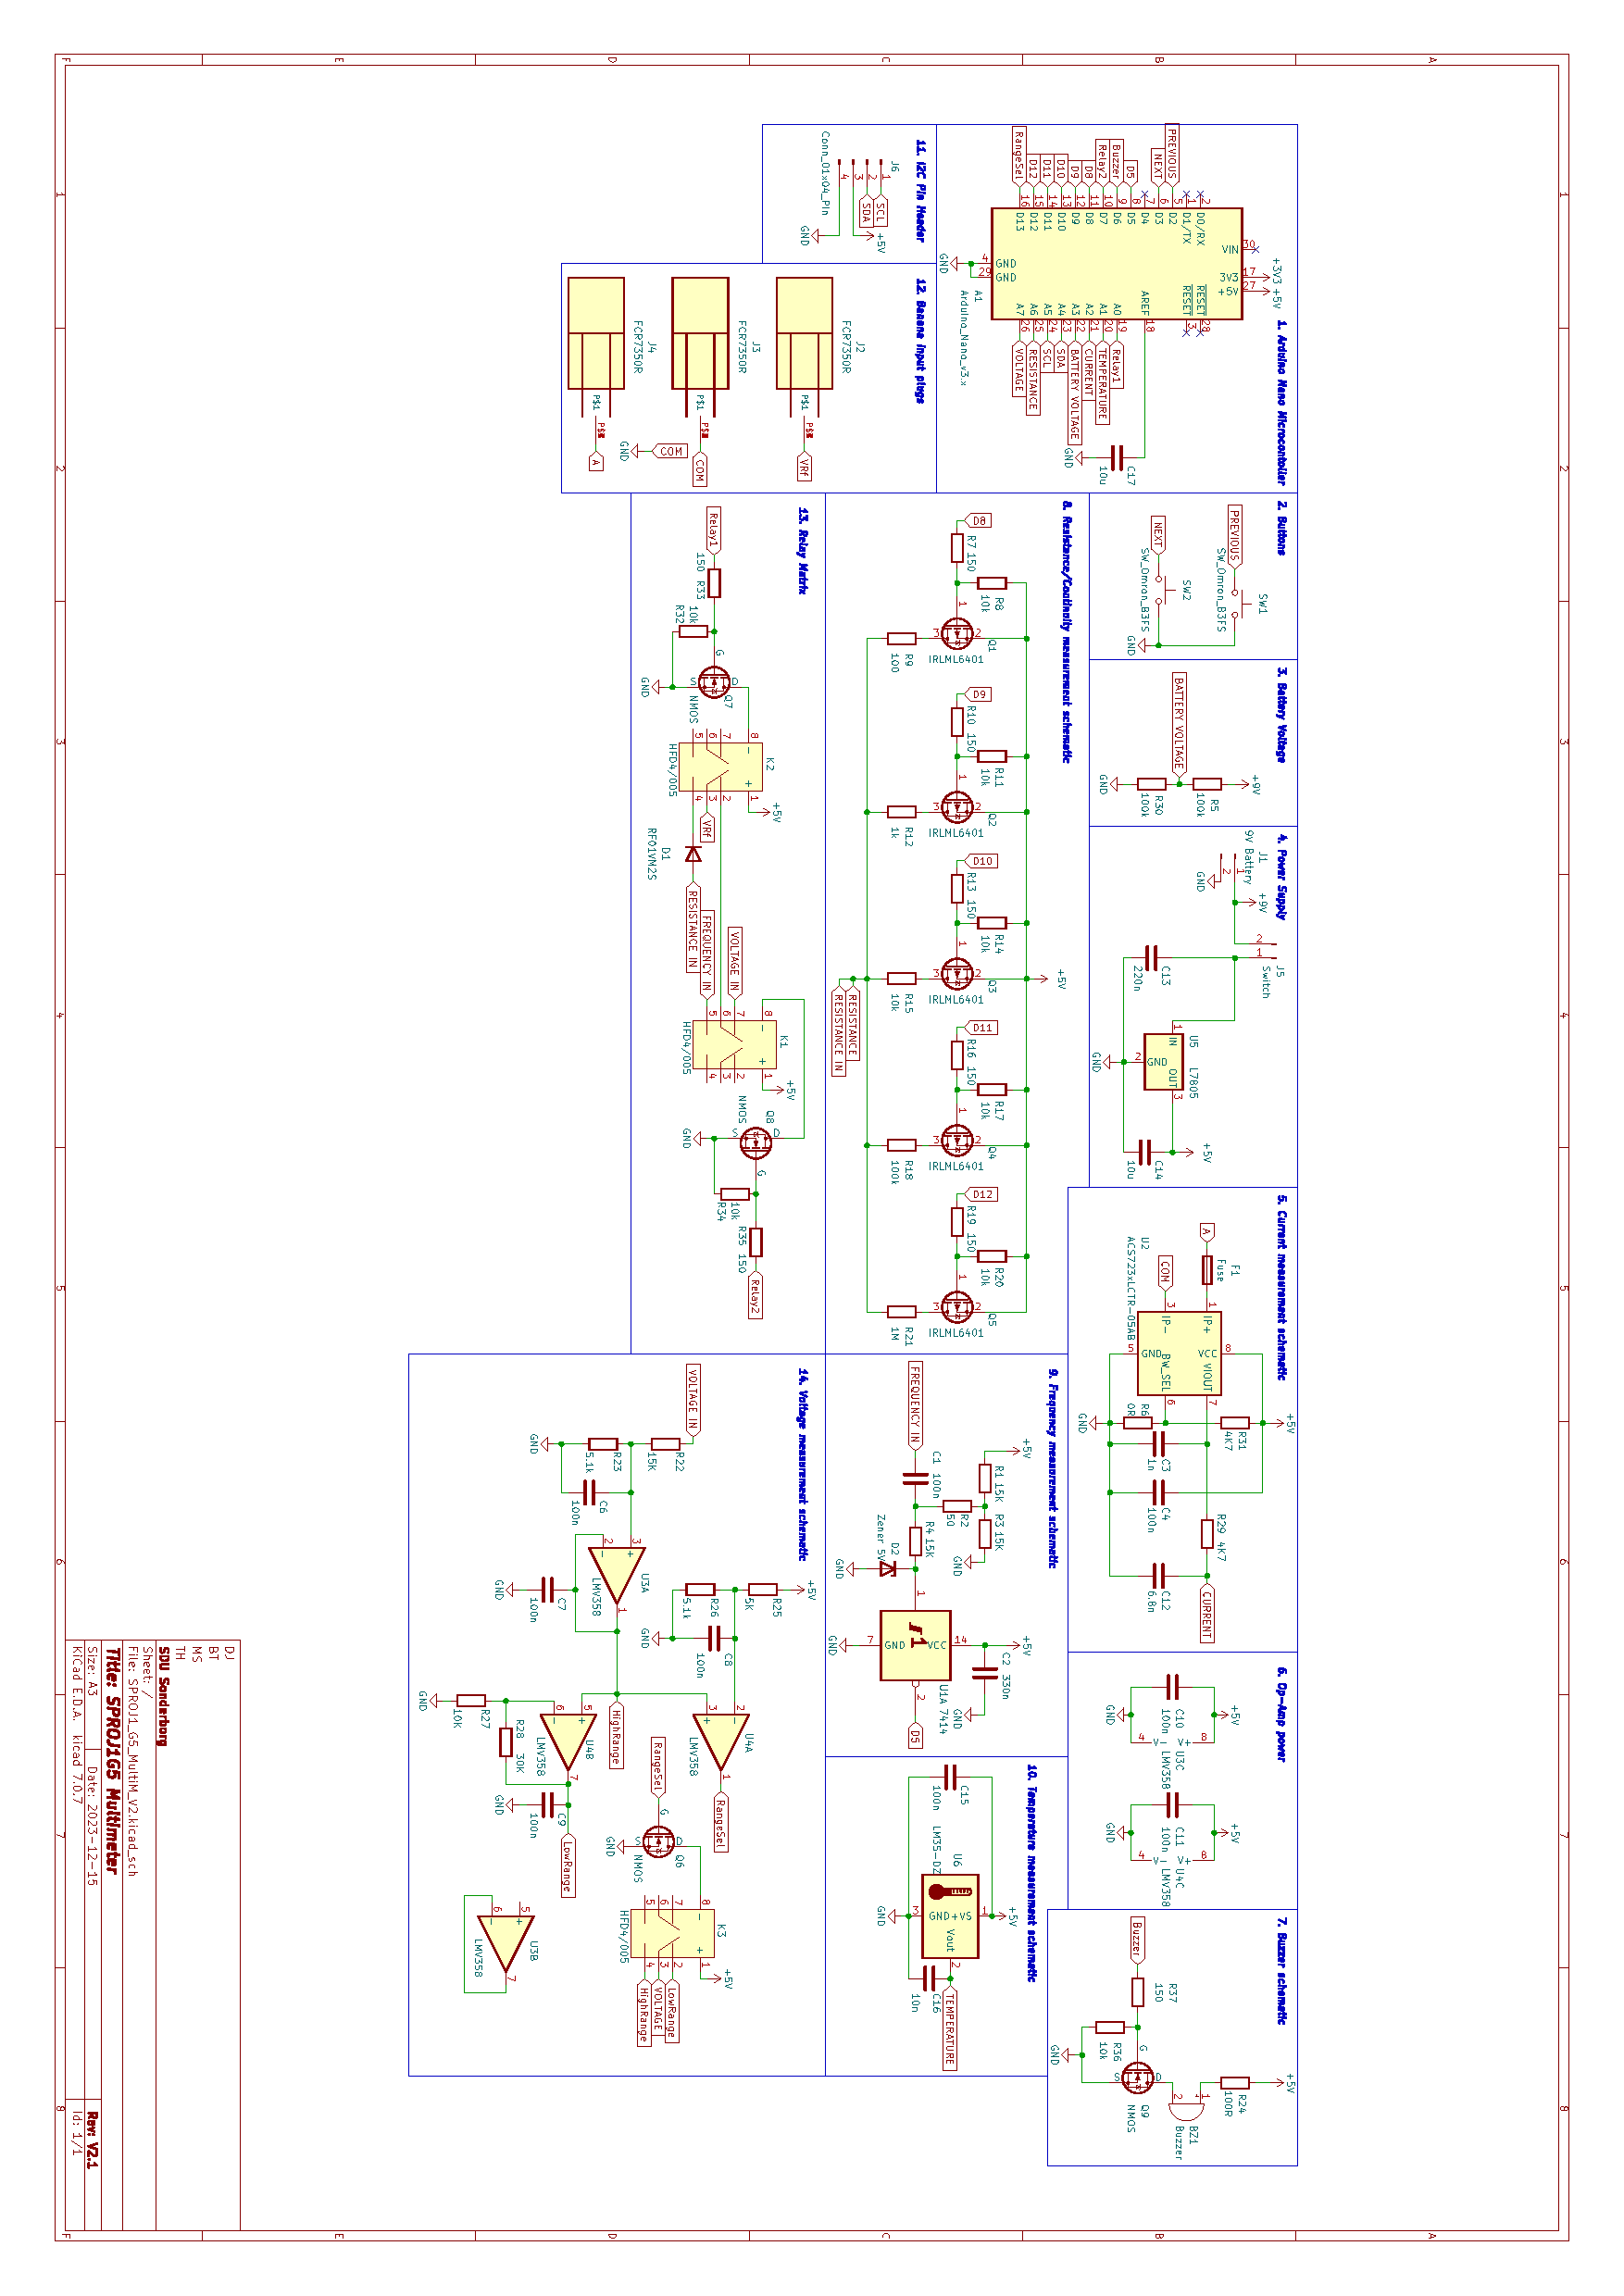
\includepdf[pages={1}]{Appendix/SPROJ1_G5_MultiM_V2.pdf}
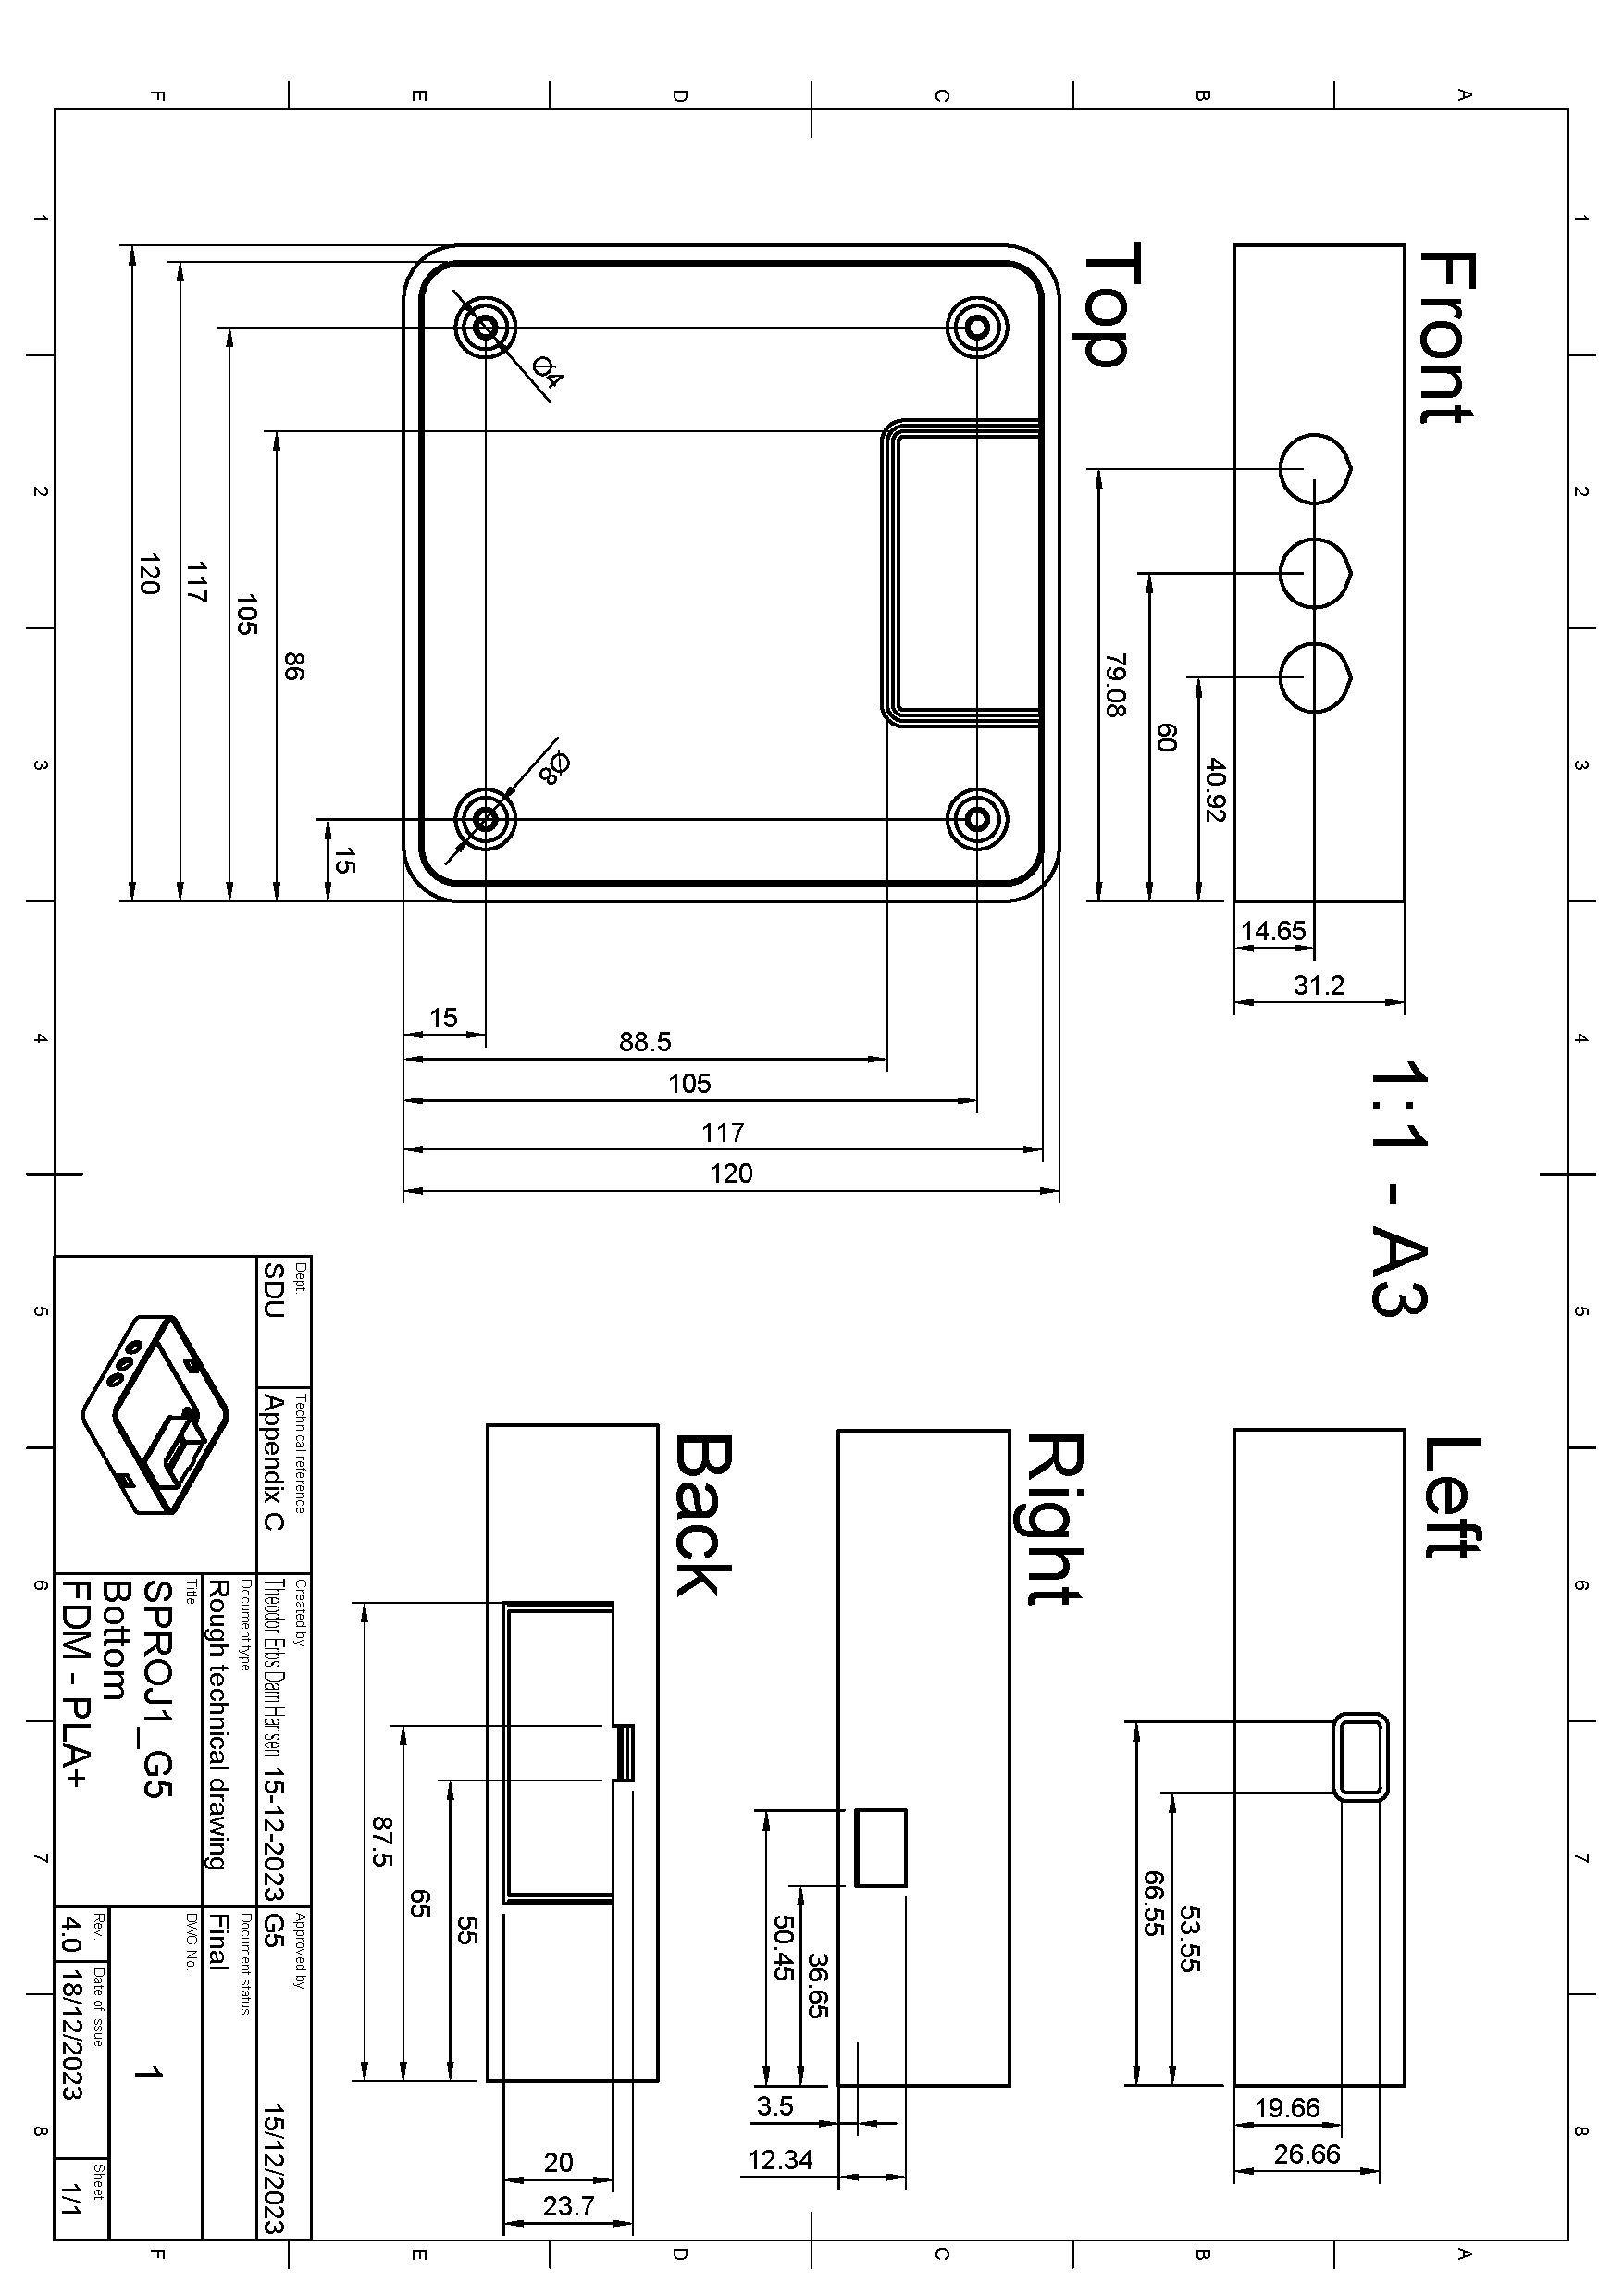
\includepdf[pages={1}]{Appendix/SPROJ1_SPIN02 Drawing v4.pdf}
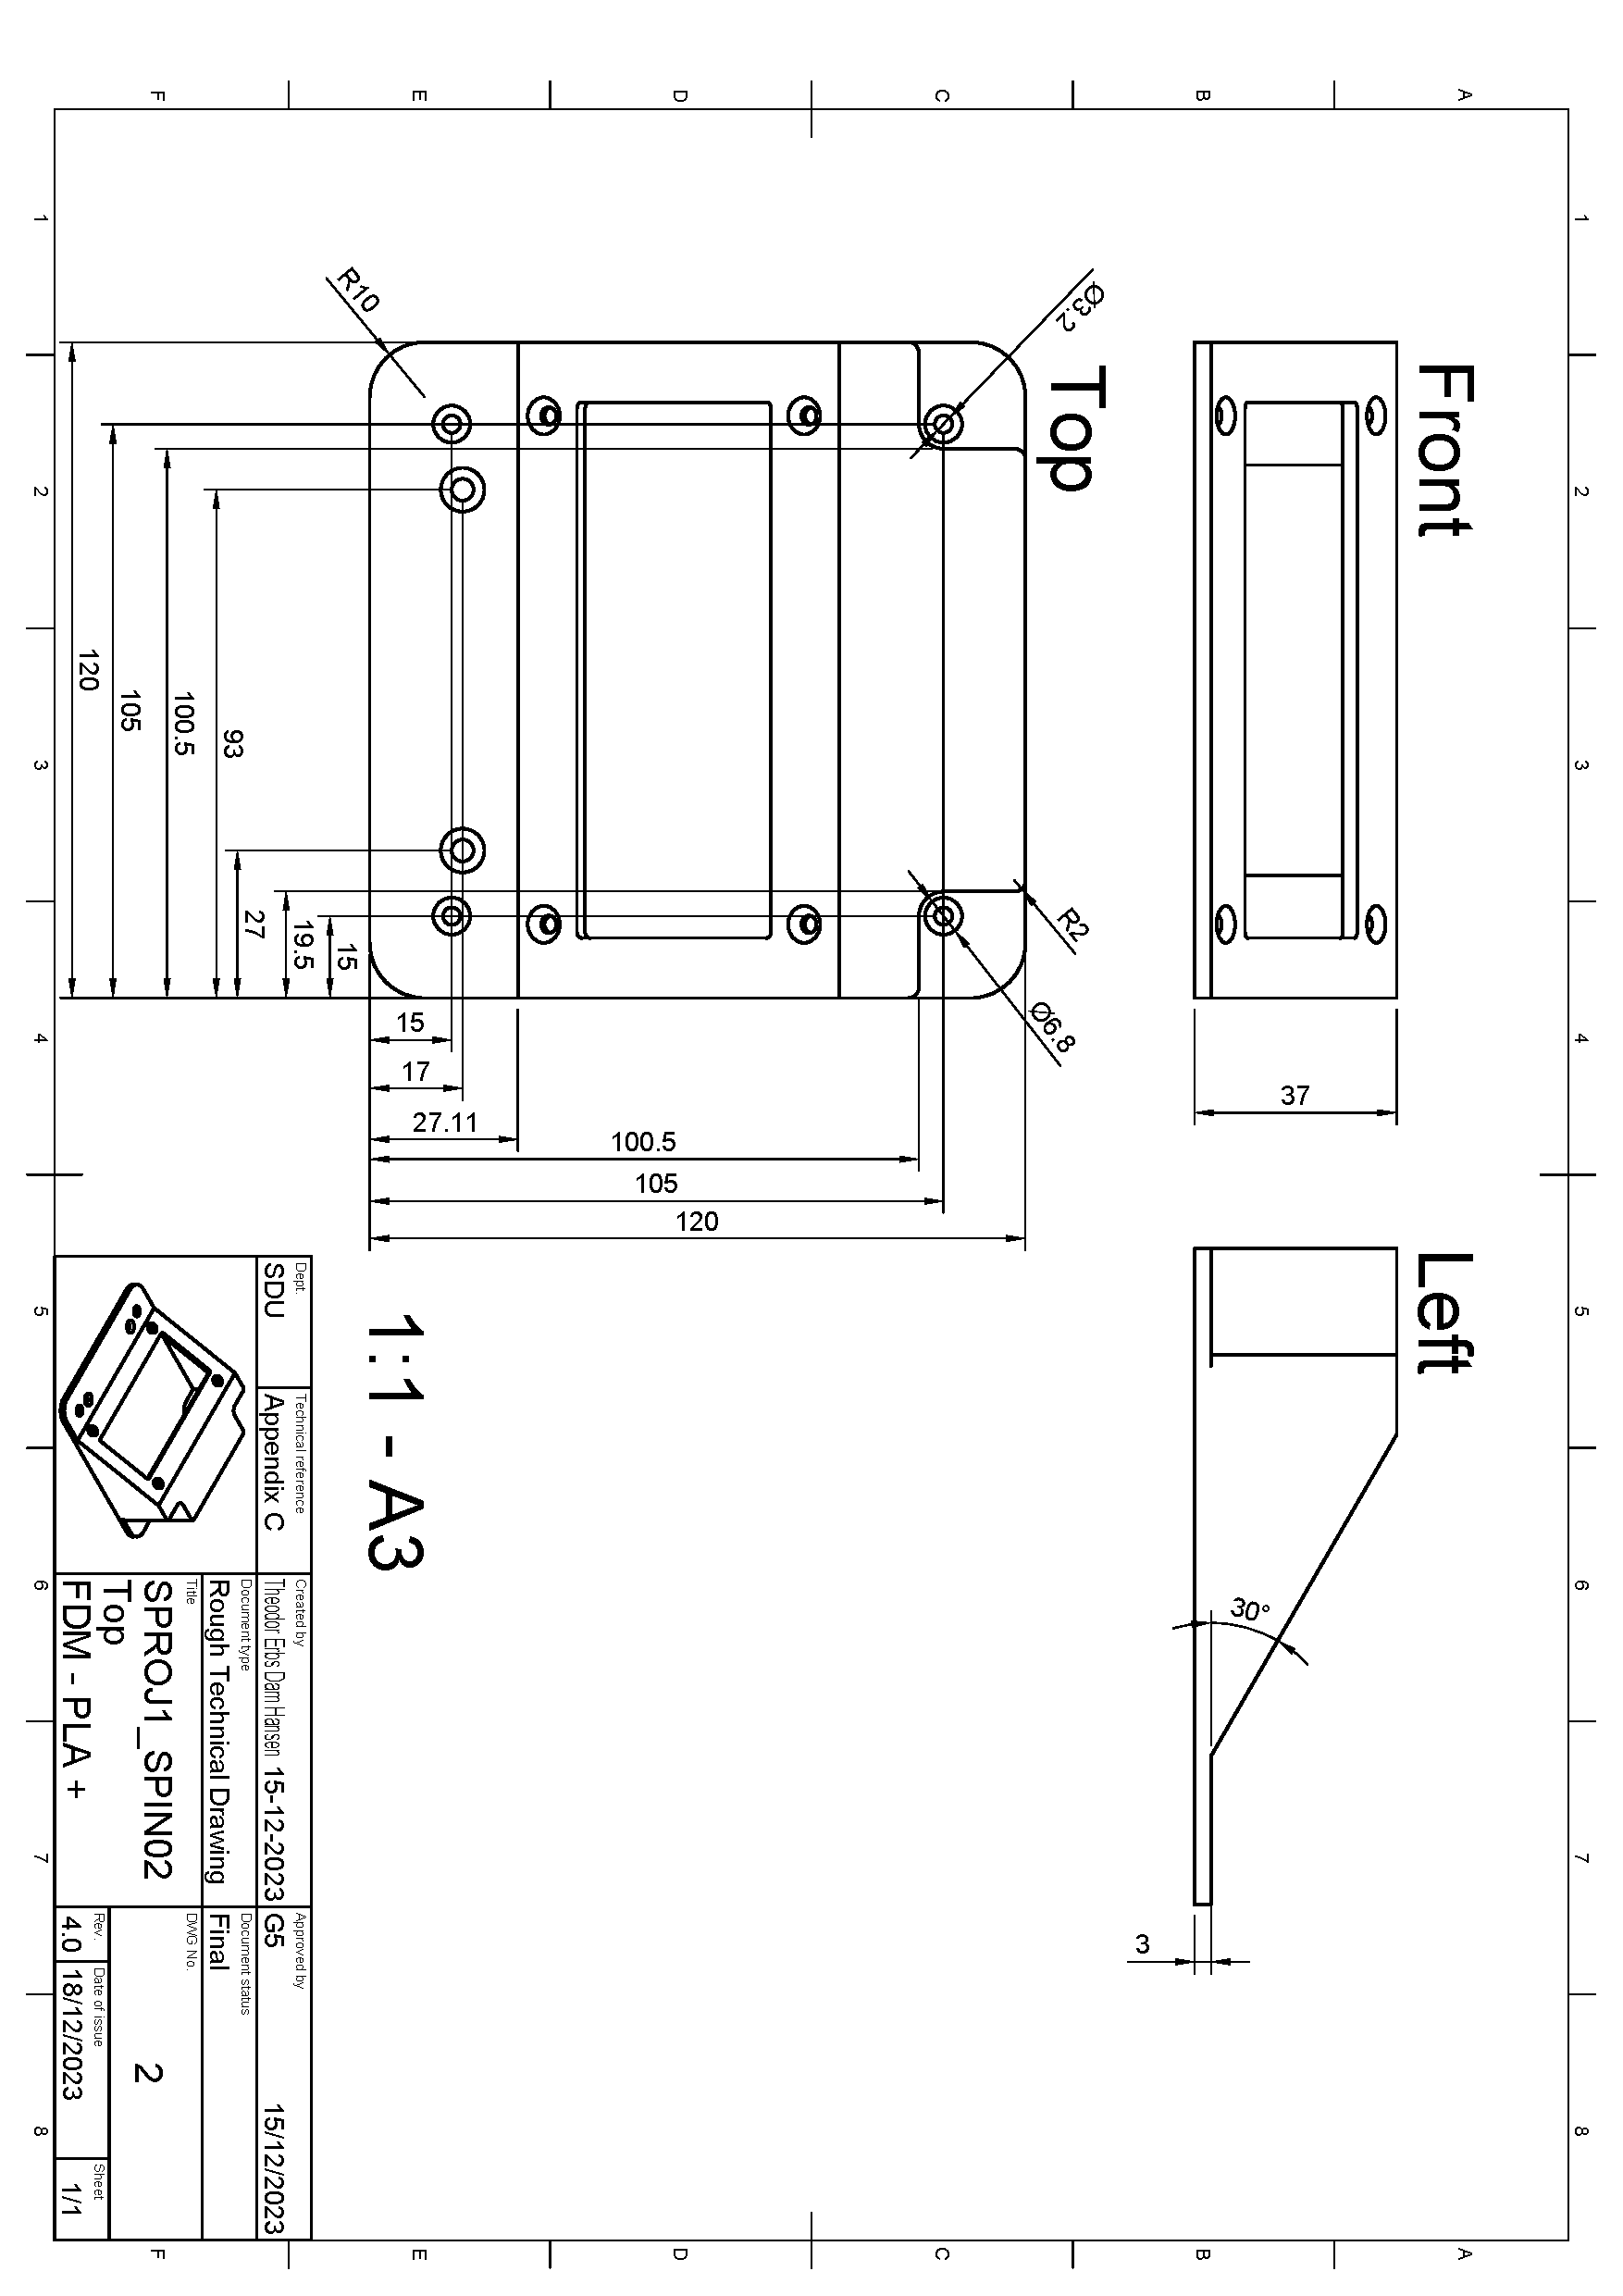
\includepdf[pages={1}]{Appendix/SPROJ1_SPIN02 Drawing top v6.pdf}
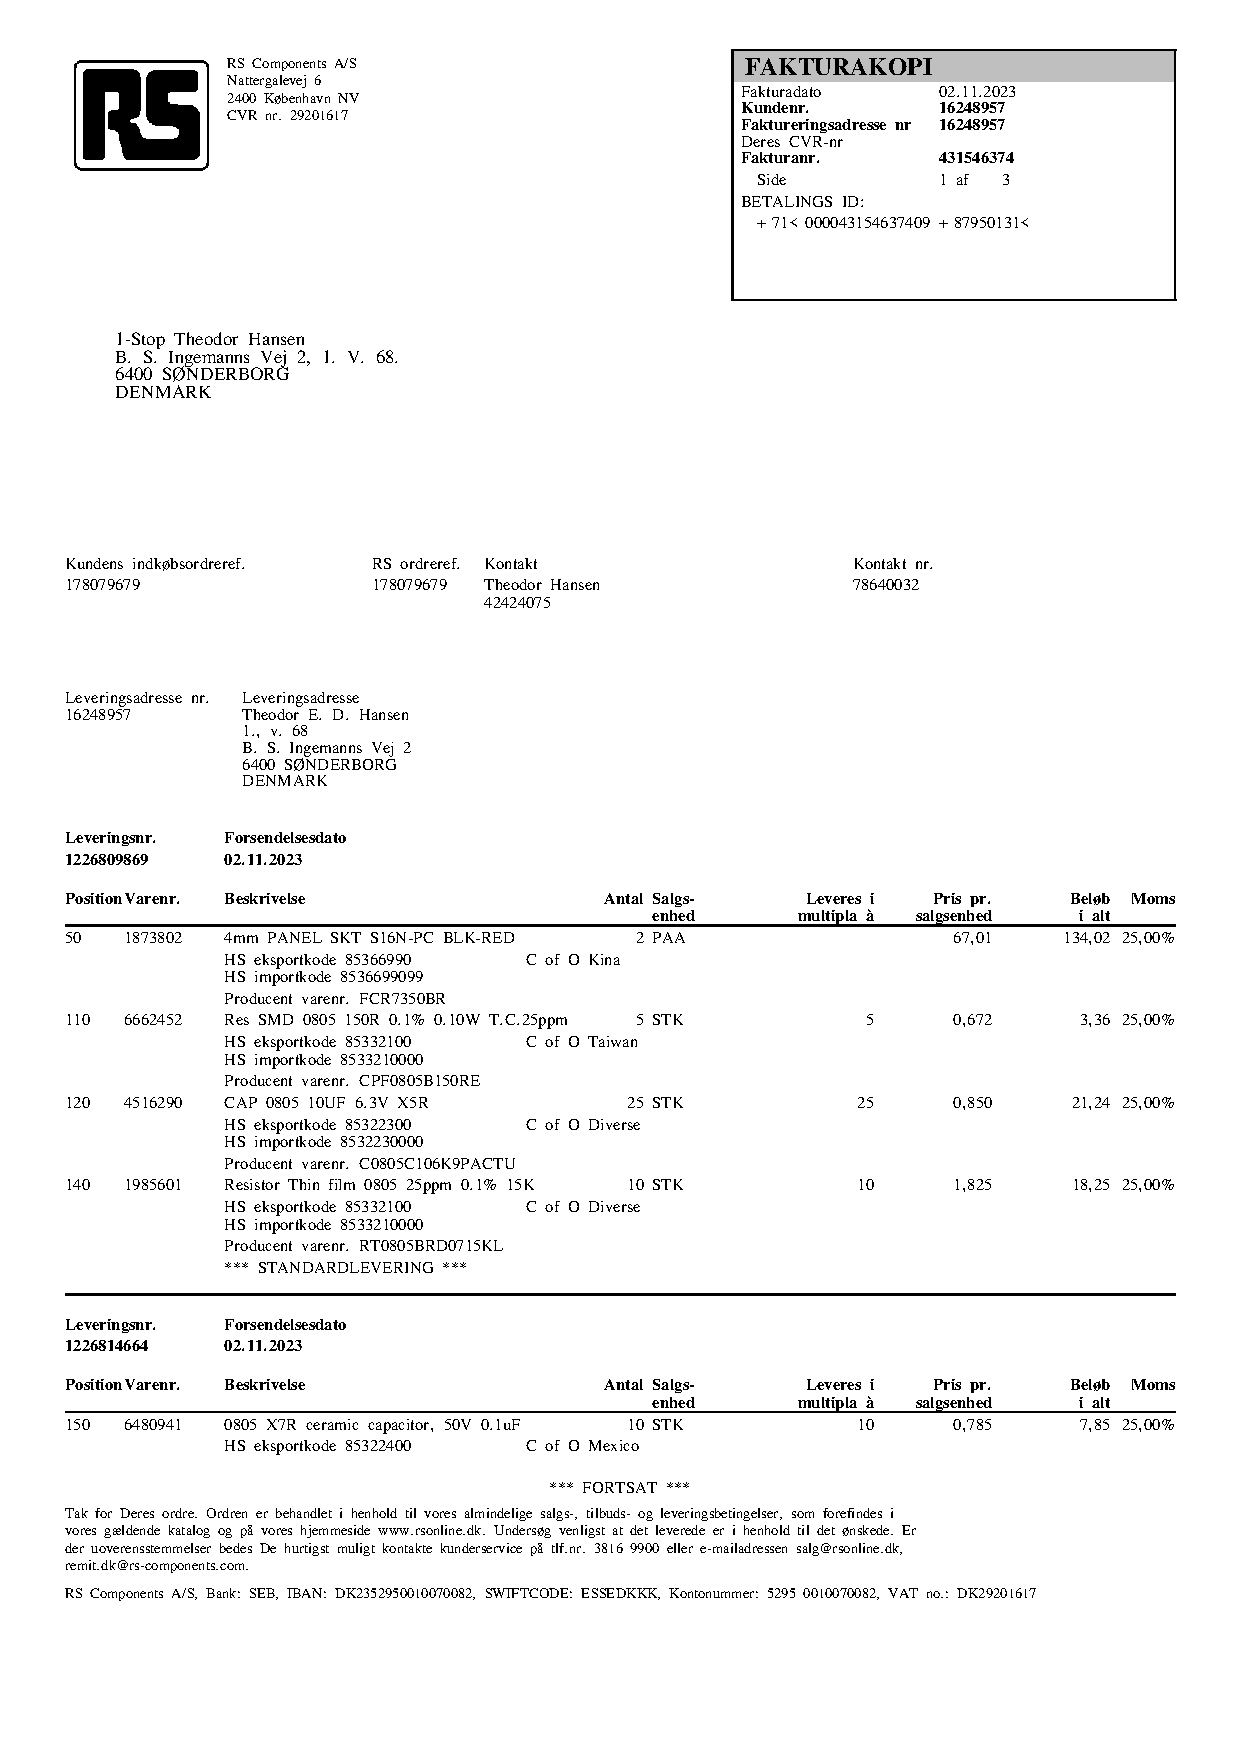
\includepdf[pages=-]{Appendix/BOM_RS.PDF}
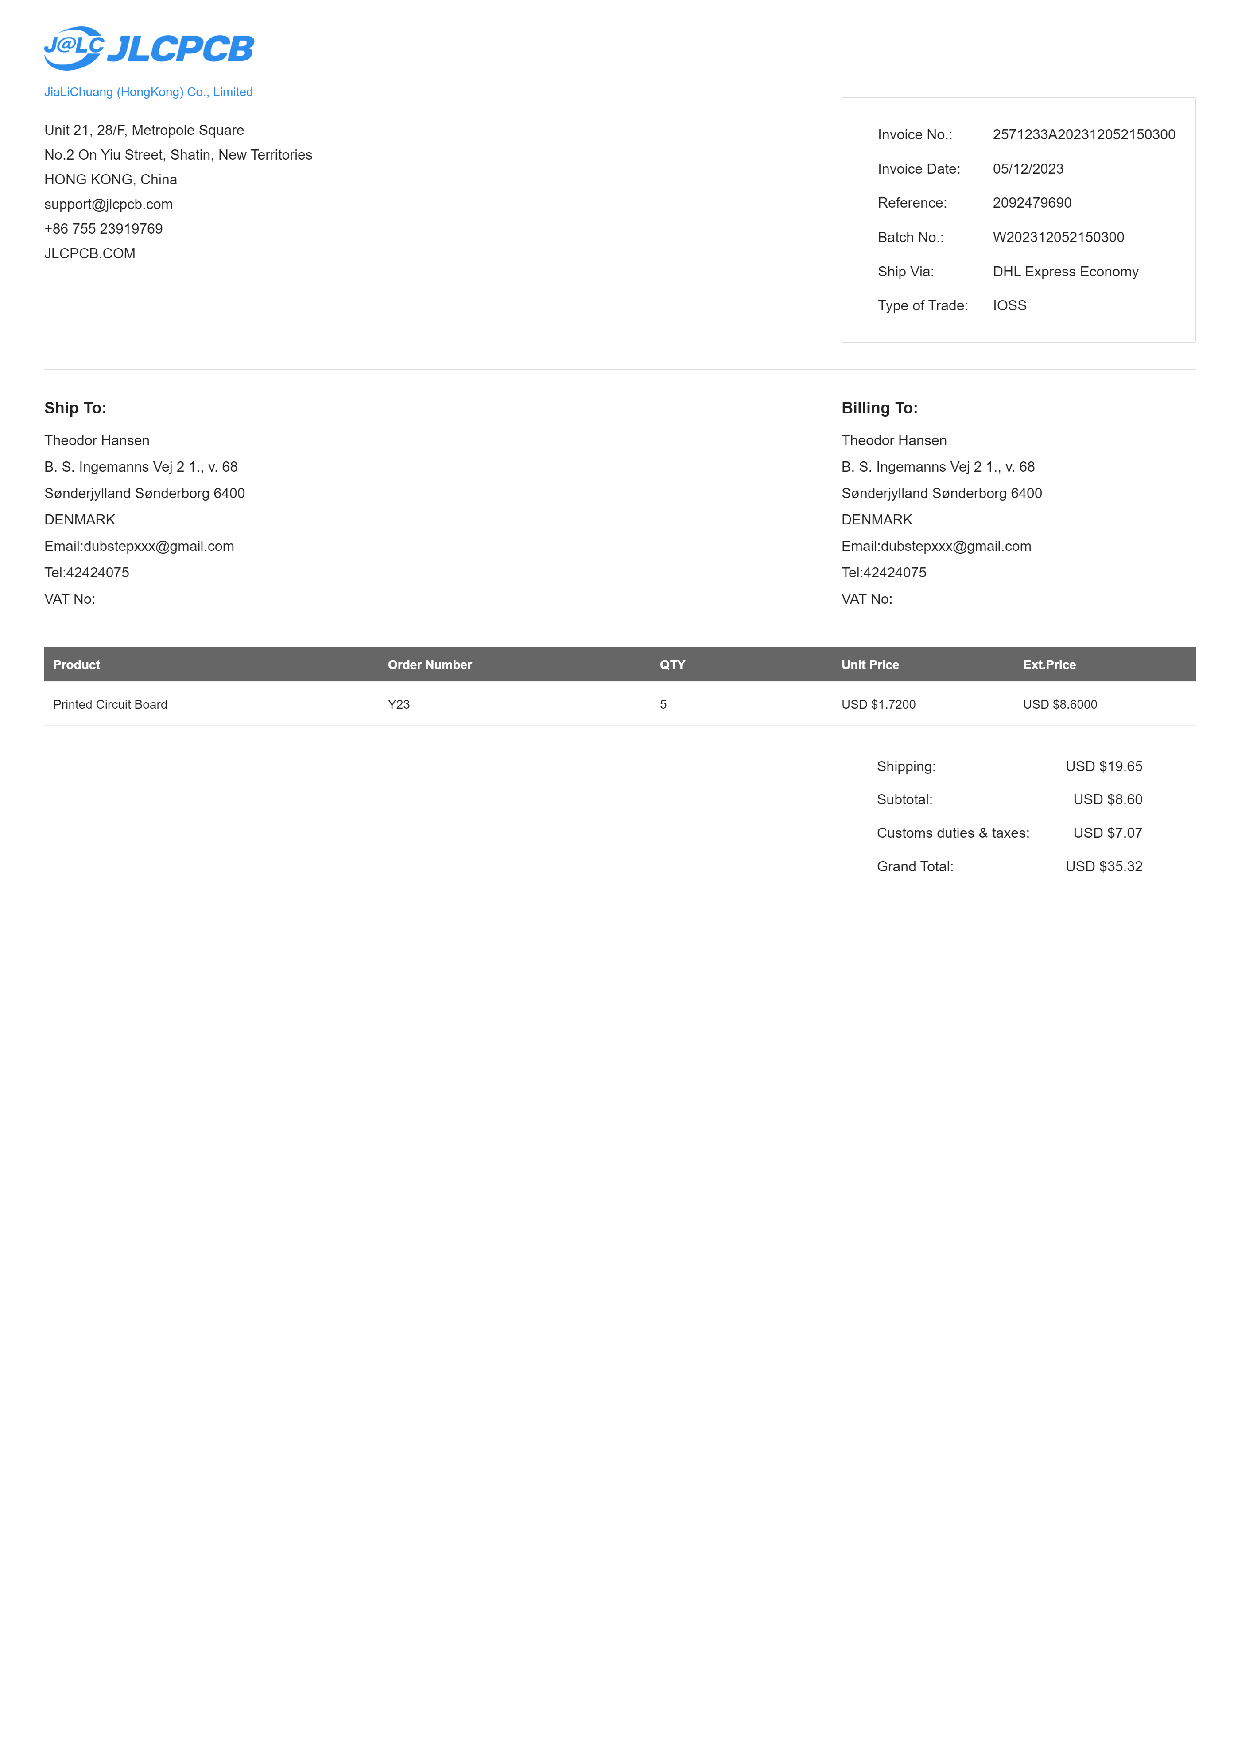
\includepdf[pages=-]{Appendix/JLCPCB_invoice.pdf}